\chapter
 [Qoala: an Application Execution Environment for Quantum Internet Nodes]
 {Qoala: an Application Execution Environment for Quantum Internet Nodes}
\label{chp:qoala}

\begin{abstract}
Executing quantum internet applications presents unique challenges not encountered in quantum computing.
These challenges include the need for a highly interactive execution of hybrid classical-quantum programs running at different network nodes, where the limited lifetime of quantum memories imposes deadlines to achieve a desired level of performance. What's more, part of the execution is subject to strict timing constraints (e.g. entanglement generation), while others allow more flexible timing precision (e.g. classical messages exchanged between the nodes). 
Here, we present Qoala, the first execution environment for programmable nodes in a quantum internet to address these challenges including:
(1) A unified program format for hybrid interactive classical-quantum programs, providing a well-defined target for compilers, and 
(2) A runtime representation of a program that allows joint scheduling of the hybrid classical-quantum program, multitasking, and asynchronous program execution.
Based on concrete design considerations, we put forward the architecture of Qoala, including the program structure and execution mechanism.
We implement Qoala in the form of a modular and extendible simulator that is validated against real-world quantum network hardware (available online).
However, Qoala is not meant to be purely a simulator, and implementation is planned on real hardware.
We evaluate Qoala's effectiveness and performance sensitivity to latencies and network schedules using an extensive simulation study.
Qoala provides a framework that opens the door for future computer science research into quantum network applications, including scheduling algorithms and compilation strategies that can now readily be explored using the framework and tools provided. 
\end{abstract}

\section{Introduction}
\label{qoala:sec:introduction}

\begin{figure}% [ht]
    \centering
    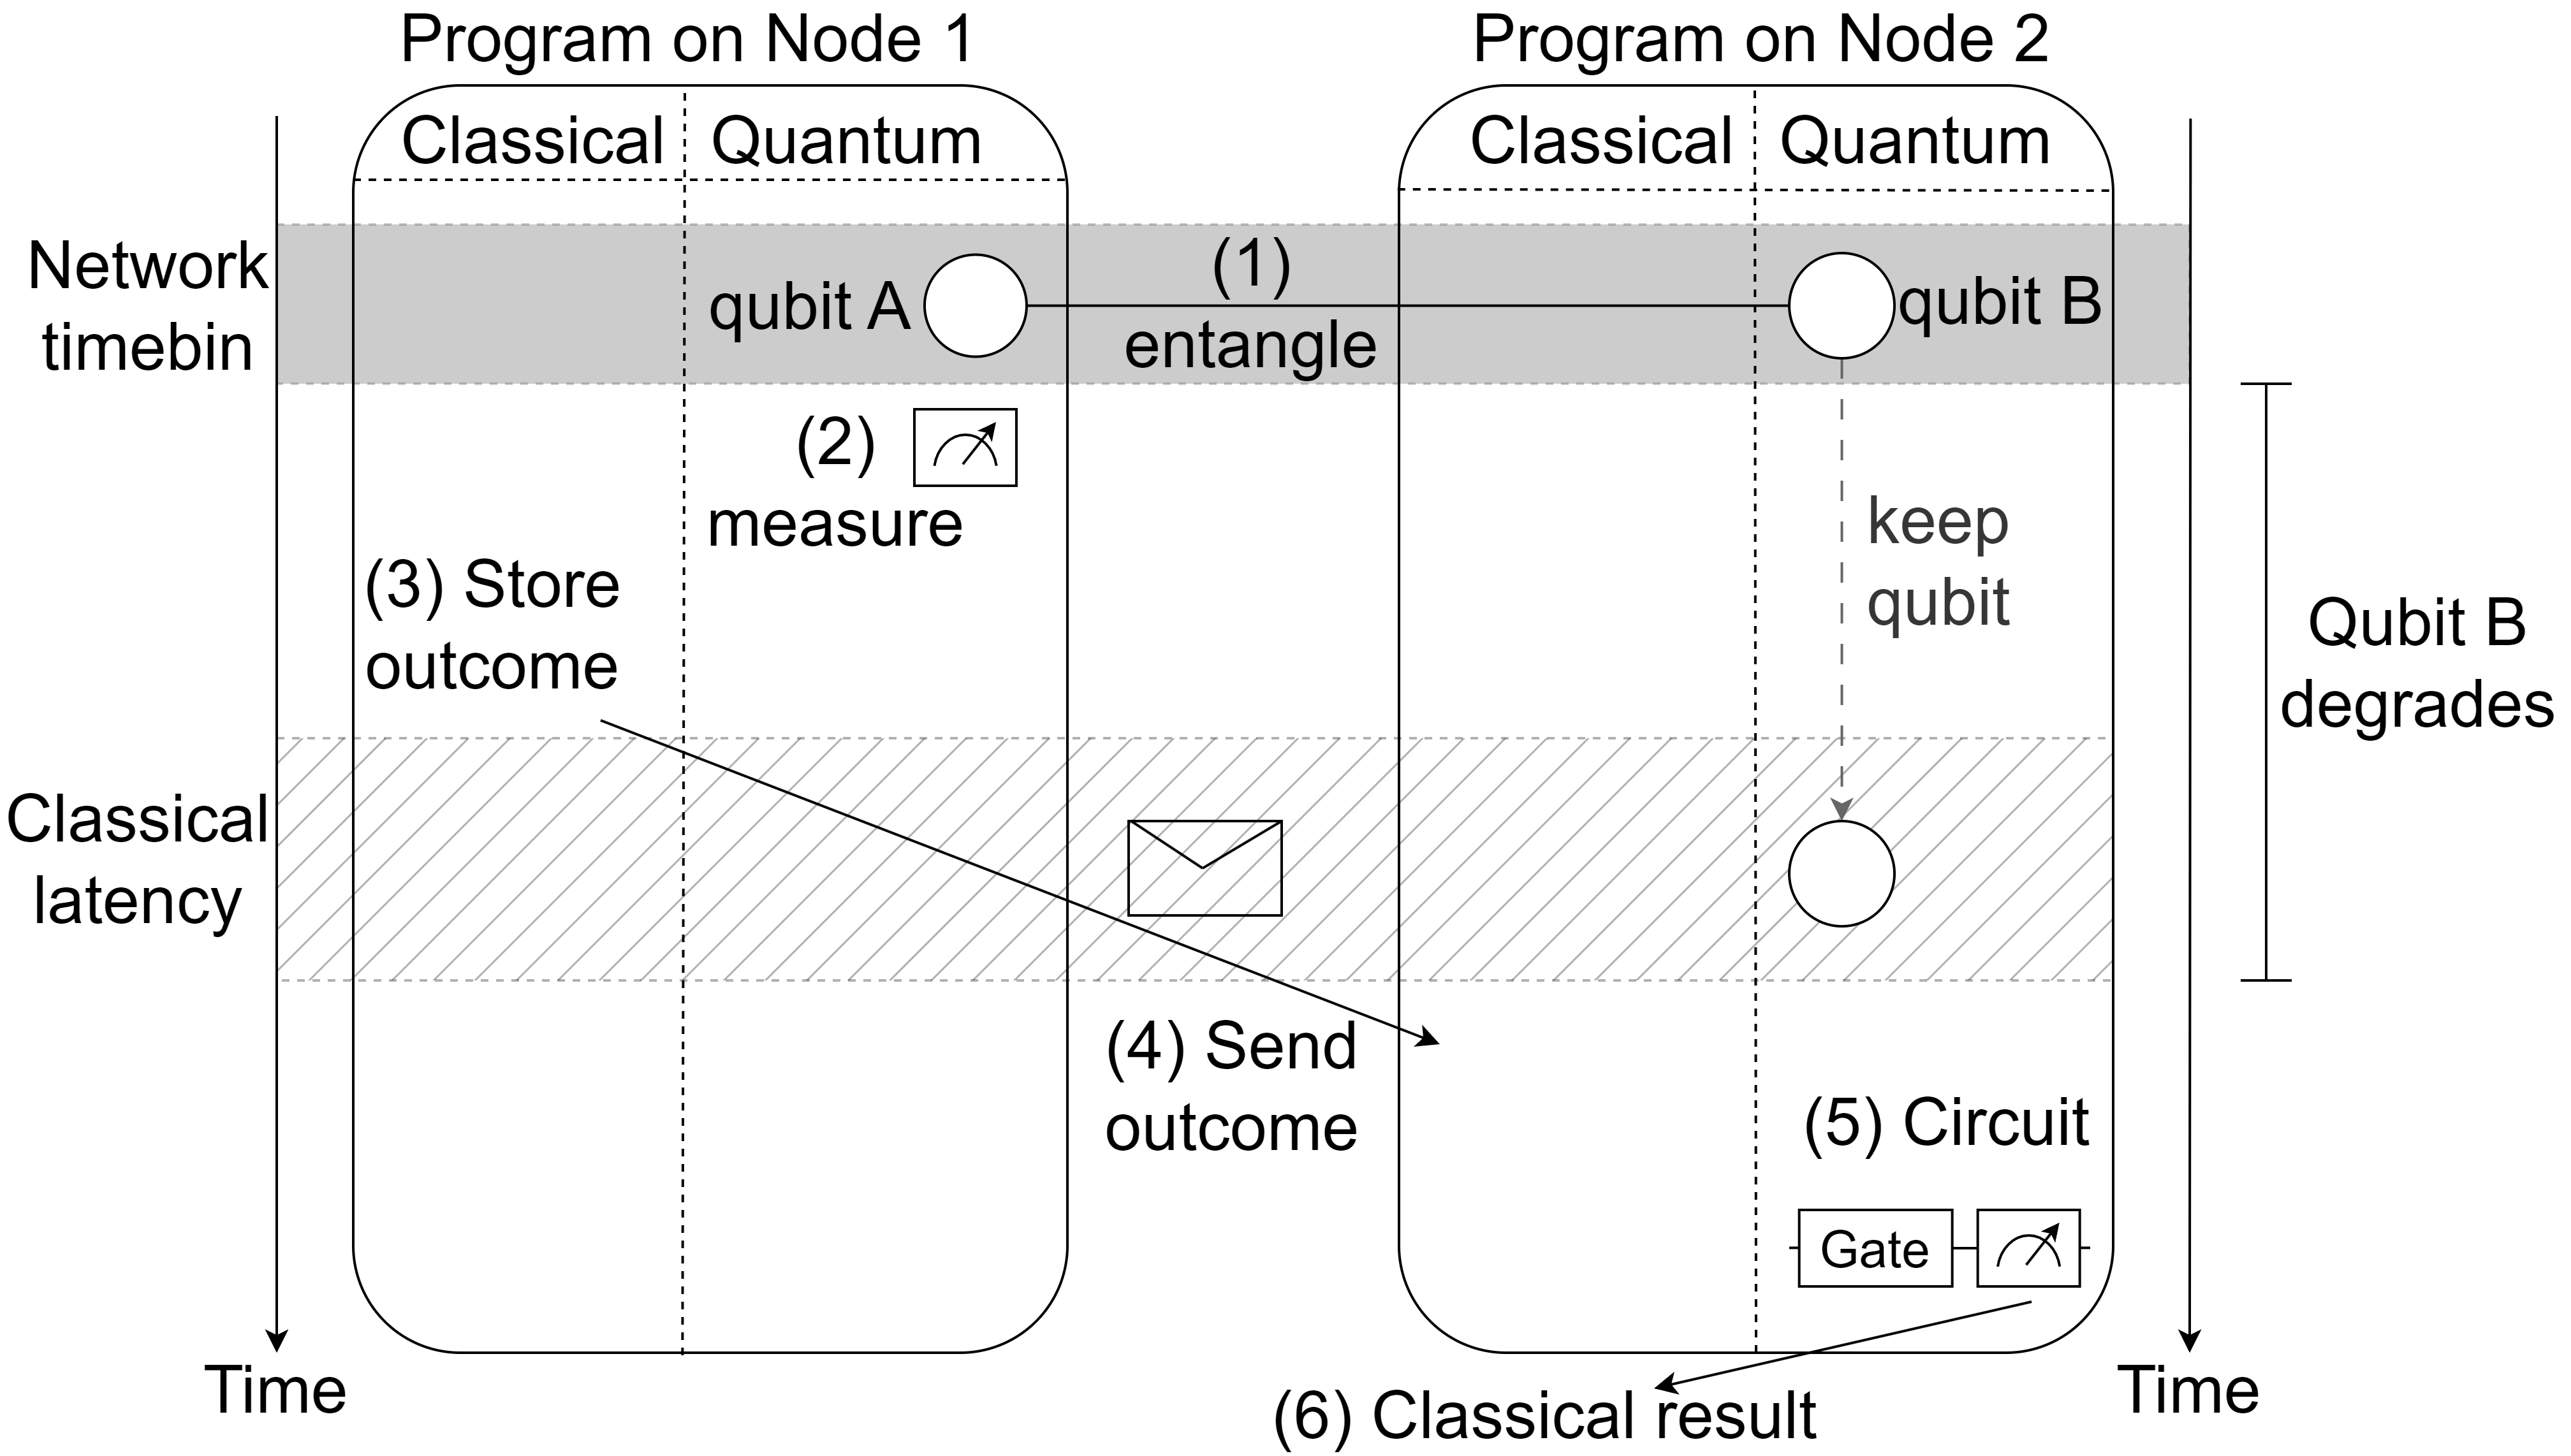
\includegraphics[scale=0.35]{figures/qoala/program_illustration.png}
    \caption{Example application consisting of two hybrid classical-quantum programs (on Nodes 1 and 2) including
        (1) Entanglement generation between two qubits (circles) in a synchronized time slot (defined by  network controller).
        (2) A local measurement of qubit A at Node 1 resulting in a classical outcome bit (destroying the qubit)
        (4) Communication of the classical bit from Node 1 to Node 2 (taking non-deterministic time)
        (5) Execution of a quantum circuit on qubit B at Node 2 depending on the classical bit. The quality of qubit B has degraded during the time elapsed since (1). 
        (6) Node 2 measures qubit B and outputs the classical result.
    }
    \label{fig:program_illustration}
\end{figure}


Advances in quantum computing and quantum communication technologies are paving the way for a \textit{quantum internet}~\cite{wehner2018quantum, kimble2008quantum}, where quantum applications are executed across multiple network nodes.
Examples of such applications include quantum key distribution (QKD)~\cite{bennett2014quantum, ekert1991quantum} and blind quantum computation (BQC) \cite{broadbent2009universal, arrighi2006blind} from a client to a quantum cloud server.
A multi-node quantum internet application is partitioned into separate single-node \textit{programs} (e.g. a client program and a server program in BQC) that run concurrently on different network nodes. To support security sensitive applications, each program performs local classical and quantum computations on its own private node, and programs interact with each other only via classical message passing and entanglement generation. This is in sharp contrast to distributed quantum computing (see e.g.~\cite{cacciapuoti2019quantum}), where all nodes can be accessed and controlled by a single program. 

The single-node programs that constitute a quantum internet application are hybrid in nature (see Fig~\ref{fig:program_illustration}):
First, they contain quantum operations, such as local quantum gates and measurements (e.g. to perform a server computation in BQC), and entanglement generation (e.g. to produce key in QKD). Entanglement is a special property of two quantum bits (qubits) that forms a key resource for quantum internet applications. 
All quantum operations are executed on quantum processors that can store, manipulate and measure quantum information, where small networks including such processors have been realized using different quantum hardware platforms including, for example,  Nitrogen-Vacancy (NV) centers in diamond~\cite{pompili2021realization}, and Ion Traps~\cite{krutyanskiy2023entanglement}.
Second, programs need to perform classical operations, such as message passing (e.g., a BQC client program sending desired measurement bases to the BQC server), and local classical processing (e.g., post-processing measurement outcomes in QKD).

Realizing the execution of quantum internet applications presents unique challenges (see Section~\ref{qoala:sec:design_considerations}): 
First, a program for a quantum internet application is not merely a hybrid of classical and quantum code segments; these segments are also highly \textit{interactive}: classical and quantum code may run concurrently, communicating and influencing each other.
E.g., a quantum circuit may "pause" halfway, keeping quantum states in memory, and wait for a value from a classical segment (e.g. a classical message from a remote node) before continuing.
Quantum memories have limited lifetimes, meaning qubits are subject to decoherence, degrading their quality over time. This introduces the need 
control the joint schedule of the classical and quantum segments of the program to reach desired levels of application performance.

Second, a compiler should be able to optimize the whole program including both classical and quantum code, as well as to provide information that can be used in our architecture to align and inform scheduling decisions. 

Finally, we are faced with a mix of time scales:
on the one hand, entanglement generation requires a very precise network schedule that is agreed ahead of time between the network nodes~\cite{dahlberg2019link}. On the other hand, classical messages are exchanged asynchronously between the nodes without guaranteed message delivery times. This motivates an architecture in which different segments of the system may operate at different levels of timing precision. 

\subsection{Main contributions}
We propose the first architecture, Qoala, that addresses these challenges. Qoala is an execution environment tailored to programmable quantum internet nodes, accommodating the \textbf{hybrid, interactive, networked, and asynchronous nature} of quantum internet applications. 

\textbf{Unified program format for hybrid-classical quantum programs:}
Qoala defines a unified program format for executables, encompassing classical and quantum (networked and local) code, and defining basic blocks.
This paves the way for a joint optimization of the classical and quantum code by a compiler.
% The program format is also made such that it can be the output of a compiler, making use of basic blocks.

\textbf{Runtime representation allowing scheduling:} Qoala separates the static unified program format from a runtime representation consisting of \textit{tasks}. 
This paves the way to design and implement algorithms for scheduling the quantum program in order to meet deadlines imposed by decoherence of the quantum memory.  
To provide advice to the scheduler on deadlines to achieve a desired program performance, programs can specify advice for timing and prioritization depending 
on the quantum hardware capabilities of the node. 
The separation of a static program from its runtime tasks also allows for the programmer to define asynchronous code segments, the execution of which is decided by the scheduler alone.
This is the first architecture that allows for effective scheduling control of hybrid interactive classical-quantum programs, thus addressing a critical issues in the successful execution of quantum internet applications.

\textbf{Integration with quantum network stack:}
Qoala integrates with an existing quantum network stack~\cite{dahlberg2019link} implemented on NV centers in diamond~\cite{pompili2022experimental} for realizing entanglement generation between nodes. This opens the door for Qoala to be implemented on such networks.

\textbf{Implementation in hardware validated simulation:} We implement the proposed architecture as a \textbf{modular and composable simulator}, which enables the evaluation of different execution strategies and techniques.
The simulation is validated against real-world quantum hardware implementations, opening the door to understand performance tradeoffs and requirements for Qoala's implementation. Specifically, the simulator allows 
configuring different hardware parameters, latencies, and software component organizations, to evaluate implementation choices of Qoala in simulation. 

Using the implementation we demonstrate the effectiveness and feasibility of our proposed architecture on different types of quantum hardware, including its ability to schedule and multitask applications using a number of existing scheduling methods (EDF, FCFS).
We continue to examine tradeoffs in the classical and quantum performance metrics of using different types of scheduling approaches. 
We examine Qoala's improvement over NetQASM~\cite{dahlberg2022netqasm} in enabling hybrid classical-quantum compilation possibilities. 
Finally, we study trends in application performance when varying the amount of concurrency, and examine the impact of a network schedule for entanglement generation on the performance of Qoala.

We highlight the role of Qoala in opening the door for computer science research. We make our simulator available as open source~\cite{qoala2023simulator}, paving the way for computer scientists to conduct further research, e.g., into the design of compilers, or schedulers that can readily be tested using the simulator. 

The remainder of this paper is structured as follows. Section~\ref{qoala:sec:related_work} compares our work to related studies. In Section~\ref{qoala:sec:design_considerations} we explain important context and terminology, followed by considerations that we used to design our architecture (Section~\ref{qoala:sec:architecture}). Section~\ref{qoala:sec:implementation} discusses our implementation and Section~\ref{qoala:sec:evaluation} provides evaluation results using this implementation. We conclude and give suggestions on future work (Section~\ref{qoala:sec:conclusion}).


\section{Related work}
\label{qoala:sec:related_work}

Networks of quantum processors have been realized using different quantum hardware platforms including, for example, nitrogen-vacancy (NV) centers in diamond~\cite{pompili2021realization}, and trapped ions~\cite{krutyanskiy2023entanglement}.
A first operating system QNodeOS~\cite{donne2024design} (see also \cref{chp:qnodeos}) including a network stack~\cite{pompili2022experimental} has been designed and implemented on real quantum network nodes based on NV centers in diamond.
QNodeOS makes use of the NetQASM execution framework~\cite{dahlberg2022netqasm} (see also \cref{chp:netqasm}), where a classical network processing unit (CNPU) dispatches NetQASM routines for execution by a quantum network processing unit (QNPU).
This meant, e.g., that QNodeOS was unable to have any scheduling control over the joint classical-quantum execution, which could lead to a failure in executing programs successfully.
Our work builds on top of ideas of QNodeOS and NetQASM, but addresses critical challenges that were not handled by these previous systems, including the ability to schedule hybrid programs and to optimize over the whole program code (see \cref{qoala:fig:qoala_vs_qnos} for a comparison).
Building on the only such systems that have seen real world implementation on quantum hardware, opens the door for a later implementation of Qoala on quantum hardware by implementing an improved low-level classical control hardware architecture (\cref{qoala:sec:architecture}).

\begin{figure}[t]
    \centering
    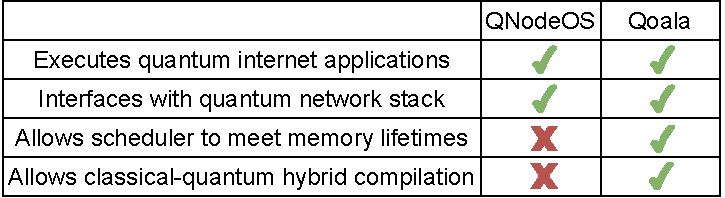
\includegraphics[width=0.7\textwidth]{figures/qoala/qoala_vs_qnos.pdf}
    \caption{
        QNodeOS (\cref{chp:qnodeos}) vs. Qoala capabilities.
    }
    \label{qoala:fig:qoala_vs_qnos}
\end{figure}

Research has been done on related topics, such as distributed quantum computing, or hybrid (non-interactive) quantum computing. Hybrid classical-quantum programs have been extensively studied in quantum computing, e.g. in the context of \textit{variational quantum eigensolvers (VQE)}~\cite{diadamo2021distributed, liu2022layer} or \textit{quantum approximate optimization algorithms (QAOA)}~\cite{farhi2014quantum}. However, they differ in two important aspects: although they are hybrid, they are not \textit{interactive} during the quantum execution:
(1) classical and quantum segments do not run concurrently, but quantum segments are executed in their entirety before returning to classical segments, i.e. no quantum state is kept in the processor between the execution of different quantum segments.
(2) such hybrid programs lack network interoperability (entanglement generation and classical message-passing between nodes), and also do not have the same timing and flexibility requirements.

Distributed quantum computing~\cite{cacciapuoti2019quantum} shares similarities with quantum internet applications but differs in several aspects.
In the former, complete control is assumed over all participating nodes, such as an application distributed across multiple cores on a single chip~\cite{ovide2023mapping, jnane2022multicore}.
Generally, the capabilities of each core and the latencies between them are fully known, allowing for precise scheduling and orchestration of individual programs running on each core to optimize overall execution.
In contrast, programs in quantum internet applications operate independently (and may even be running on different quantum hardware); therefore they have a degree of autonomy in their own scheduling, and are not fully aware of the actions or timing of other programs.

Entanglement distribution in networks is another related topic that has been extensively studied (see e.g. surveys~\cite{wei2022towards, azuma2021tools}).
However, these works do not deal with executing network applications, and give only predictions for applications in which entanglement is immediately measured (e.g. QKD).

The concept of (soft) deadlines for program execution is of course well known from classical real-time systems that are often used in domains where deterministic and time-critical response is essential, such as automotive, aerospace and medical devices~\cite{liu1973scheduling, hambarde2014survey, buttazzo2011hard}, including examples of systems with mixed timing precision~\cite{burns2017survey}.
We draw inspiration from this domain, and the present architecture opens the door to explore algorithms and concepts from this domain to be applied to the execution of quantum internet applications.

\section{Design considerations}
\label{qoala:sec:design_considerations}

\subsection{Background and context}
\label{qoala:sec:background_context}

We first revisit some of the relevant background and context (see also \cref{chp:background}).

\textit{Quantum nodes}.
A quantum internet connects quantum nodes on which quantum programs may be 
executed.
%(\cref{qoala:fig:qoala_location}). 
In their most general form, such nodes
are \textit{processing nodes} that have a quantum memory to store quantum bits (qubits) on which quantum operations (qubit initialization, quantum gates and measurements) can be performed. Pairs of nodes can establish \textit{entanglement} between them over a quantum network. Entanglement is a special property of two qubits (an \emph{entangled pair}), where one qubit is stored in the memory of each node. Nodes can also exchange classical messages (e.g. via dedicated classical links or the internet), where no guarantees are assumed on their message delivery times. 

\textit{Programs}.
A program is a series of instructions to be executed by a node.
Instructions can be categorized into four types: local classical processing, classical message-passing, quantum local processing (quantum operations), and remote entanglement generation.
A program can keep classical variables in a classical memory, and quantum variables (qubits) in the node's quantum memory during the execution.
Multiple programs, each running on their own node, together form an \textit{application} (see \cref{qoala:fig:program_illustration}), e.g. QKD (two programs, one per node),
or secret sharing~\cite{hillery1999quantum} (a program each on many nodes).
Programs may involve asynchronous operations (e.g. a server awaiting entanglement with multiple clients).

\textit{Network schedule}.
A quantum network stack has been proposed~\cite{dahlberg2019link} and implemented \cite{pompili2022experimental} that turns entanglement generation into a robust service independent of the quantum hardware platform.
Important for the design of an architecture for the execution of quantum internet applications is that in this stack, the nodes will establish a network schedule of time slots in which they will trigger entanglement generation (due to need to synchronize entanglement generation at the physical layer~\cite{dahlberg2019link} at nanosecond precision).
This means that once entanglement has been requested from the network, the nodes can use only the slots in the network schedule to produce entanglement between them, imposing constraints on the ability to schedule applications. What's more, in present day systems~\cite{pompili2021realization, krutyanskiy2023entanglement} limitations in the physical devices prohibit the execution of local operations while engaging in network operations (entanglement generation), creating further dependencies between the local quantum execution and entanglement generation. 
As the specifics of network scheduling~\cite{network-scheduling, skrzypczyk2021architecture} are not within scope of this thesis,
we assume the existence of a \textit{network controller} that takes application demand for entanglement and issues a network schedule to the nodes. 
A schedule consists of sequential time slots, each with a start time and duration, when the node will trigger entanglement generation.
Nodes are not forced to attempt entanglement in corresponding time slots, and can instead choose to do local processing instead.


\textit{Performance metrics and noise}. Quantum internet applications have classical outcomes that are typically probabilistic in nature:
(1) applications may intentionally do measurements on quantum states that have fundamentally probabilistic outcomes (e.g. quantum cryptography),
(2) in practice, quantum hardware is imperfect (or \textit{noisy}). That is, undesired errors occur
when performing operations (such as gates, measurements, or entanglement generation) or when keeping quantum states in memory for too long.

In many quantum internet applications (e.g. BQC), a single execution of the application can result in failure or success (e.g. a BQC client receives correct measurement results from the server program~\cite{leichtle2021verifying}). Applications are often executed many times, where outcome statistics are computed in order to validate successful execution (e.g. by majority of outcomes).
We consider two metrics:
a \emph{quantum metric} --- the \textit{success probability} of executing a single instance of the application (on average), and a \emph{classical metric} --- the \textit{makespan}, i.e. the average execution time of an application instance.

\subsection{Considerations}
Considerations can be categorized into three main groups: fundamental, technological, and enabling.

\noindent\textit{\textbf{Fundamental Considerations}}
(1) \textit{Hybrid nature of applications (FC1)}: Quantum internet applications inherently consist of both classical and quantum segments, as well as local and networking operations. The execution environment must account for this hybrid nature, and the program structure should accommodate all types of operations.
(2) \textit{Interactive nature of applications (FC2)}: Quantum internet applications require classical communication between nodes. This communication may take place in between classical and quantum segments of a single program. 
This implies the need for application-level interfaces between programs on different nodes, and for interfaces between classical and quantum code segments on a single node.
(3) \textit{Multitasking (FC3)}: Programs may spend a significant amount of time waiting for messages from a remote node (ms), motivating multitasking to make optimal use of the classical and quantum computing resources at each node.  This requires scheduling of time and resources.

\noindent\textit{\textbf{Technological Considerations}}
(1) \textit{Limited qubit lifetime (TC1)}:
Quantum memory quality degrades over time, presenting a significant challenge for the execution environment,
especially in near-term hardware (ms to s memory lifetimes~\cite{ruf2021quantum, pompili2021realization, krutyanskiy2023telecom}).
As such, there are natural deadlines to application execution after which a desired performance (success probability) can no longer be reached.
We thus desire that a program specification allows indication of memory quality constraints (deadlines), which the runtime environment can act upon (e.g. by appropriate scheduling or restarting).
(2) \textit{Integration of processing and networking (TC2)}: We assume that near-term nodes only have a single quantum processor, which needs to perform both local quantum gates as well as remote entanglement generation.
That is, while performing local operations the processor is blocked from networking operations and vice versa, as is the case for all current implementations~\cite{pompili2021realization, krutyanskiy2023entanglement} but may be mitigated partially using future proposals~\cite{vardoyan2022quantum}. 
The node must hence allocate time for local computation while at the same time adhering to the network schedule which constrains timing of the entanglement operations.

\noindent\textit{\textbf{Enabling Considerations}}
(1) \textit{Different compilation strategies and programming languages (EC1)}: The execution environment should support various compilation strategies and accessible programming languages. 
In order to enable compilation, we furthermore want a representation of the program that can be integrated with existing compiler frameworks.
(2) \textit{Different scheduling strategies (EC2)}: Since we expect that scheduling plays a vital role in optimizing application performance, the execution environment should enable scheduling, and support different scheduling algorithms and policies, 
allowing for their comparison and evaluation.
(3) \textit{Different (control) hardware implementations (EC3)}: The architecture should make minimal assumptions on the classical control hardware, and be independent on the choice of quantum hardware platform~\cite{carlothesis},
allowing for integration with multiple (future) technologies such as NV centers~\cite{pompili2022experimental} or trapped ions~\cite{drmota2023robust}.


\section{Architecture}
\label{qoala:sec:architecture}

Based on these design considerations, we propose Qoala (see Fig.~\ref{fig:runtime_overview}), an execution environment for programmable nodes in a quantum internet. 
Provided minimal hardware assumptions are met (Section~\ref{qoala:sec:minimal_hardware_assumptions}), 
each node implements its own Qoala execution environment, supporting a specific \textit{program structure} (Section~\ref{qoala:sec:program_structure})
and implementing a specific \textit{runtime environment} (Section~\ref{qoala:sec:runtime_environment}) that is able to \textit{schedule tasks} (Sections~\ref{qoala:sec:tasks}--\ref{qoala:sec:scheduling}).
Details in Appendices~\ref{qoala:sec:app:program_structure}, \ref{qoala:sec:app:runtime_environment}, \ref{qoala:sec:app:scheduling_execution}.

\subsection{Minimal hardware assumptions}
\label{qoala:sec:minimal_hardware_assumptions}

Qoala is based on only a few core assumptions on the processing node (Figure~\ref{fig:minimal_hardware_assumptions}):

\textit{CPS-QPS distinction}. We assume the node distinguishes between a \textit{classical processing system (CPS)} managing classical computing resources (e.g. CPU, classical memory and networking), and a \textit{quantum processing system (QPS)}, responsible for executing quantum operations (gates, measurements, entanglement generation) on quantum hardware including a quantum memory as in~\cite{dahlberg2022netqasm, pompili2022experimental}.
Unlike prior work, we assume a shared classical memory is accessible to both the CPS and QPS, enabling communication between the two processing systems, addressing the interactive property of quantum internet programs.
The CPS can act as a fully-fledged classical computer, and performs application-level classical communication with other nodes as well as with a network controller who sets a network schedule.
The QPS can execute routines consisting of low-level quantum gates, basic classical control logic (branching), and entanglement generation.
This opens the door for the QPS to be based on essentially any quantum hardware platform where a specialized microcontroller is used to control the quantum hardware, and a separate microprocessor implements the CPS, where a shared memory could be realized next to the two processors on-chip.
The scheduler controls both CPS and QPS execution, and may physically be realized on either one.

\textit{Time granularity}. Both CPS and QPS are assumed to have knowledge of time, albeit operating with different timing precision ($ms$ precision for CPS mirroring node-to-node communication latencies vs. $\mu s$ and $ns$ precision needed for synchronized entanglement generation~\cite{pompili2022experimental, dahlberg2019link}.)

 \textit{Network stack}. A quantum network stack including a network layer~\cite{dahlberg2019link} is implemented on the node with which Qoala can interface. This stack can receive and fulfill requests for remote entanglement generation.
\begin{figure}
    \centering
    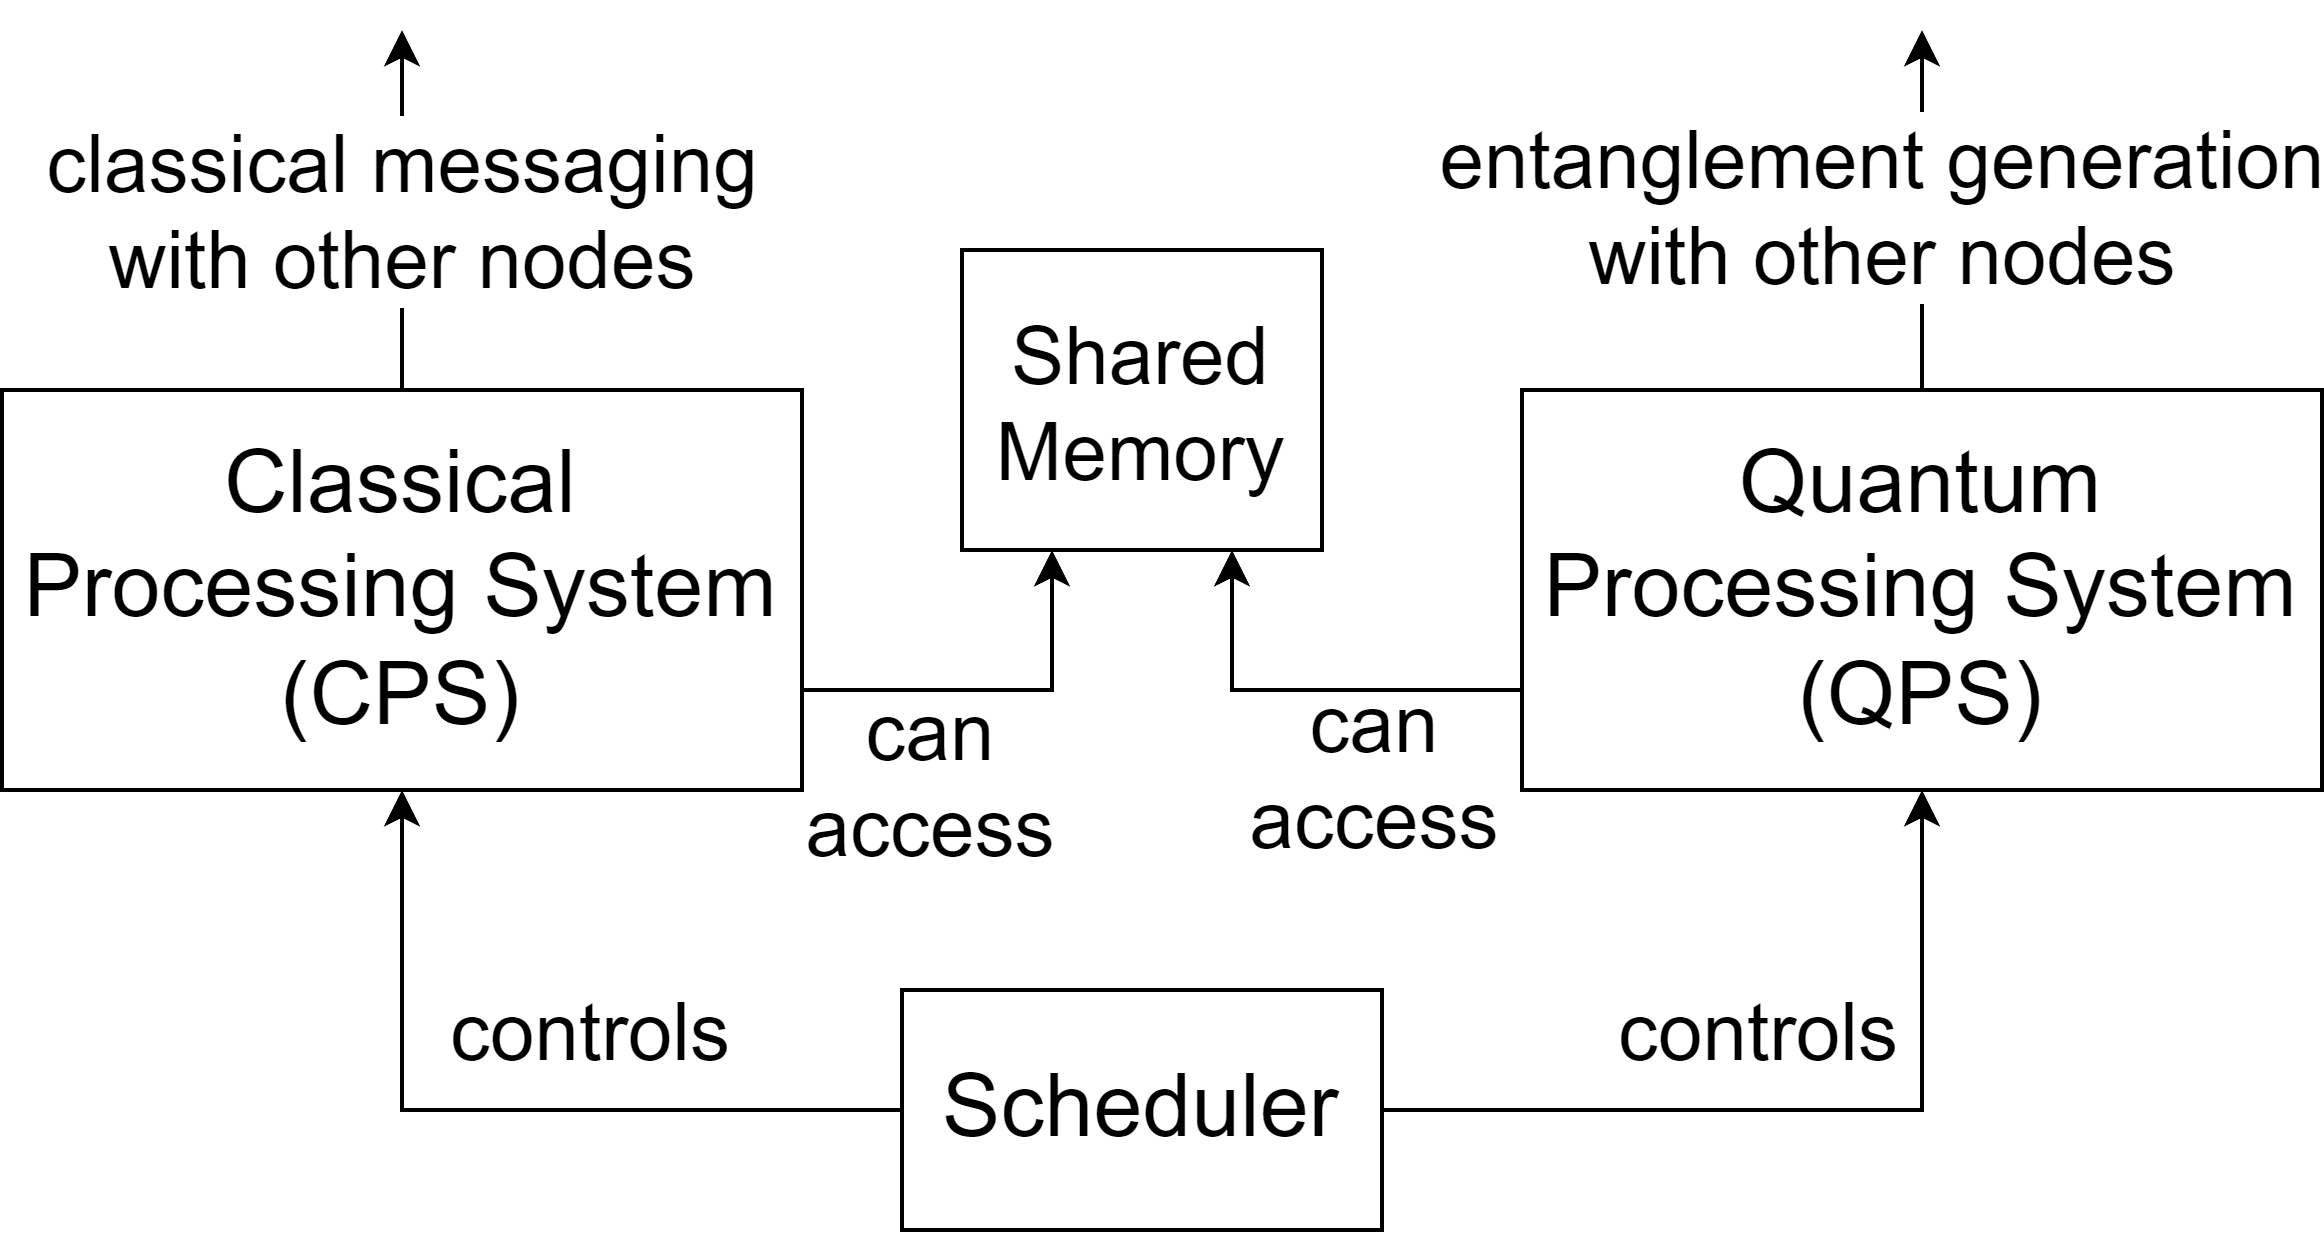
\includegraphics[width=\columnwidth]{figures/qoala/minimal-hardware.png}
    \caption{Minimal hardware assumptions for a single node.}
    \label{fig:minimal_hardware_assumptions}
\end{figure}



\subsection{Program structure}
\label{qoala:sec:program_structure}
Qoala defines a hybrid format for programs, addressing considerations in Section~\ref{qoala:sec:design_considerations}.
A Qoala program is a combination of quantum and classical instructions, 
organized into three main sections: \textit{host code} (containing classical instructions), \textit{local routines} (containing local quantum instructions), 
and \textit{request routines} (for remote entanglement generation).
This hybrid format allows a compiler to optimize the whole program, including critical code paths with dependencies between classical and quantum segments.
Local routines and request routines can be triggered from within host code as function calls, addressing the interactivity between them.

A Qoala program is an \textit{executable} and output of a compiler.
The format is separate from any high-level language in which a programmer might write code; hence Qoala in theory allows for compatibility with any such language.
Entry and exit points of a program are in host code.
Figure~\ref{fig:example_program} shows an example program in text format.
We contrast Qoala's program format with that of~\cite{dahlberg2022netqasm}, in which there was no way to compile across classical and quantum code segments.
A Qoala program has \textit{program arguments} that are filled in during program instantiation (Section~\ref{qoala:sec:program_instantiation}).


\begin{figure}%[ht]
    \centering
    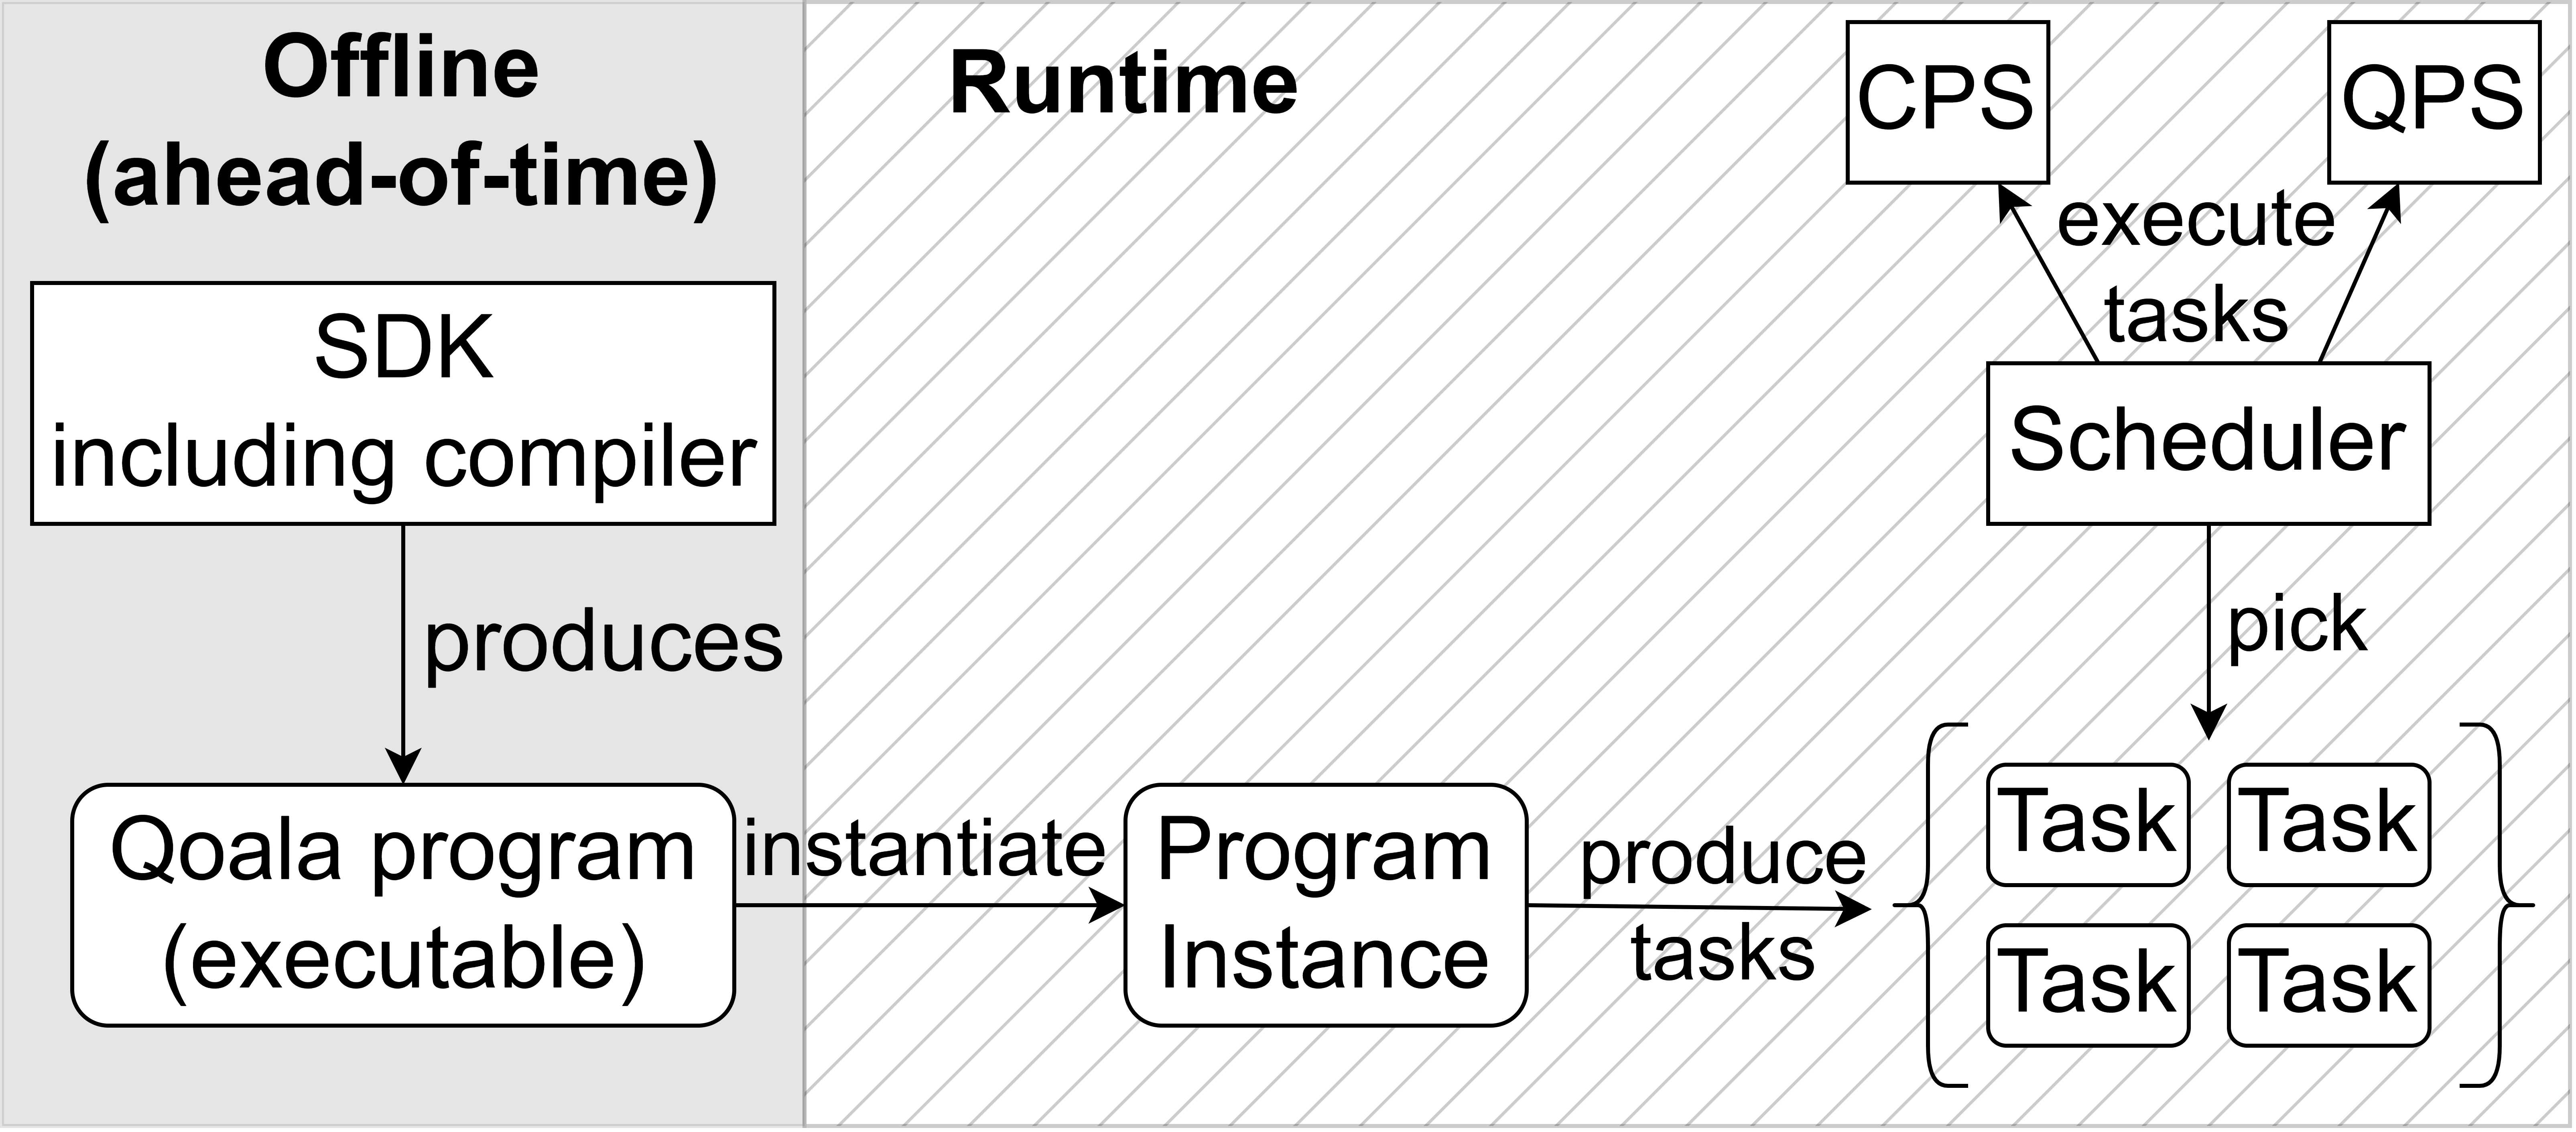
\includegraphics[width=\columnwidth]{figures/qoala/runtime_overview.png}
    \caption{High-level overview Qoala: An SDK allows program code in a high-level language (e.g. Python).
    A compiler translates this code into a Qoala program (specific compiler not in scope of this work).
    To run, a program is instantiated with concrete values for program arguments.
    Tasks are created for the program instance, which are scheduled and executed by the scheduler.
    Multiple program instances may exist at the same time (both multiple instances of the same or different programs).
    All tasks from all instances are added to a single task graph (Section~\ref{qoala:sec:tasks}) used by the scheduler.
    }
    \label{fig:runtime_overview}
\end{figure}




\textit{Host code}.
Host code, executed on the CPS, encompasses local computation, control-flow, inter-node messaging, and can initiate local and request routines.
For example, in a program that is part of a QKD application, classical post-processing (including sending bases, local error correction, and privacy amplification \cite{vidick2023introduction}) would be represented in host code.
Host code is structured as a sequence of \textit{blocks}, each holding a list of instructions.
Blocks dictate control-flow by ending with a (conditional) jump instruction (default: next block in the sequence).
This block division not only facilitates task creation and scheduling (see Section~\ref{qoala:sec:tasks}) but also streamlines compiler integration (which may use blocks in its intermediate representation).
Blocks can contain metadata about their expected \textit{duration}, (relative) deadlines, and they may be inside \textit{critical sections}, encompassing a sequence of blocks with a maximally allowed execution duration. This metadata is propagated to corresponding tasks and used by the scheduler in order to mitigate quantum decoherence due to limit qubit lifetime.
Asynchronous execution is possible by `submitting' multiple routines for execution, and waiting for all of them to finish. At runtime, the scheduler can decide in which order to execute the routines.


\textit{Local routine}.
A local routine (LR) represents a series of quantum operations (like gates and measurement), to be executed by the QPS locally (no interaction with external nodes or controllers).
An LR may also contain limited classical computation and control-flow code allowing for fast feedback, which can increase quantum performance (Section~\ref{qoala:sec:background_context}) due to less decoherence.
An updated version of NetQASM~\cite{dahlberg2022netqasm} is used to represent the instructions, which allows both hardware-specific and hardware-agnostic instructions.
Therefore, the program format is compatible with different quantum hardware.
In contrast to \cite{dahlberg2022netqasm}, Qoala's version of NetQASM does not have instructions for entanglement generation (cleanly separating local and networked quantum operations)
nor `wait' instructions. This allows routines to be treated as atomic non-preemptable blocks.
%, which makes scheduling easier).

\textit{Request routine}. A request routine (RR) consists of a request for entanglement generation with another node, and represent requests to the node's quantum network stack.
It can have local routines as callbacks, allowing quick local (quantum) processing of entangled qubits on the QPS without returning to the CPS, decreasing waiting time and decoherence.


\subsection{Runtime environment}
\label{qoala:sec:runtime_environment}
The Qoala runtime environment provides various resources that programs can leverage during execution.

\textit{Exposed Hardware Interface (EHI)}.
The Exposed Hardware Interface provides information about the hardware and software capabilities and restrictions of the node and the network,
like available quantum memory and expected latencies.
Each node provides their own EHI which is used in capability negotiation (see below), and allows a choice of executable code optimized by a compiler for those capabilities ahead of time. 

\textit{Shared memory}.
To address the classical-quantum interactivity in programs, the CPS and QPS share data with each other via \textit{shared classical memory}.
Write conflicts are avoided by explicit read/write rules for shared memory regions.
Our conceptual model of a shared memory leaves open different implementation choices, including a physical shared memory or a message-passing protocol.
Calls in host code to local or request routines use the shared memory to communicate routine arguments and results.

\textit{Quantum memory}.
Quantum memory is organized into a \textit{virtual quantum memory space (VQMS)} for each program instance (see Section~\ref{qoala:sec:program_instantiation} for instantiation), represented as Unit Modules~\cite{dahlberg2022netqasm}.
Qoala maps each VQMS to the physical qubits available in the QPS.
VQMS information like qubit connectivity and noise characteristics is provided by the EHI, which a compiler can use to optimize a program.
The VQMS enables multitasking since programs have their own runtime context, while a scheduler (Section~\ref{qoala:sec:scheduling}) sees the whole physical memory space and can schedule programs accordingly.

\textit{Remote interaction}. For interaction with programs on remote nodes,
the runtime provides \textit{classical sockets} and \textit{EPR sockets} based on~\cite{dahlberg2022netqasm}. Host code uses classical sockets for sending and receiving messages; EPR sockets are indicated in request routines (see e.g. Figure~\ref{fig:example_program}).

\begin{figure}% [ht]
    \centering
    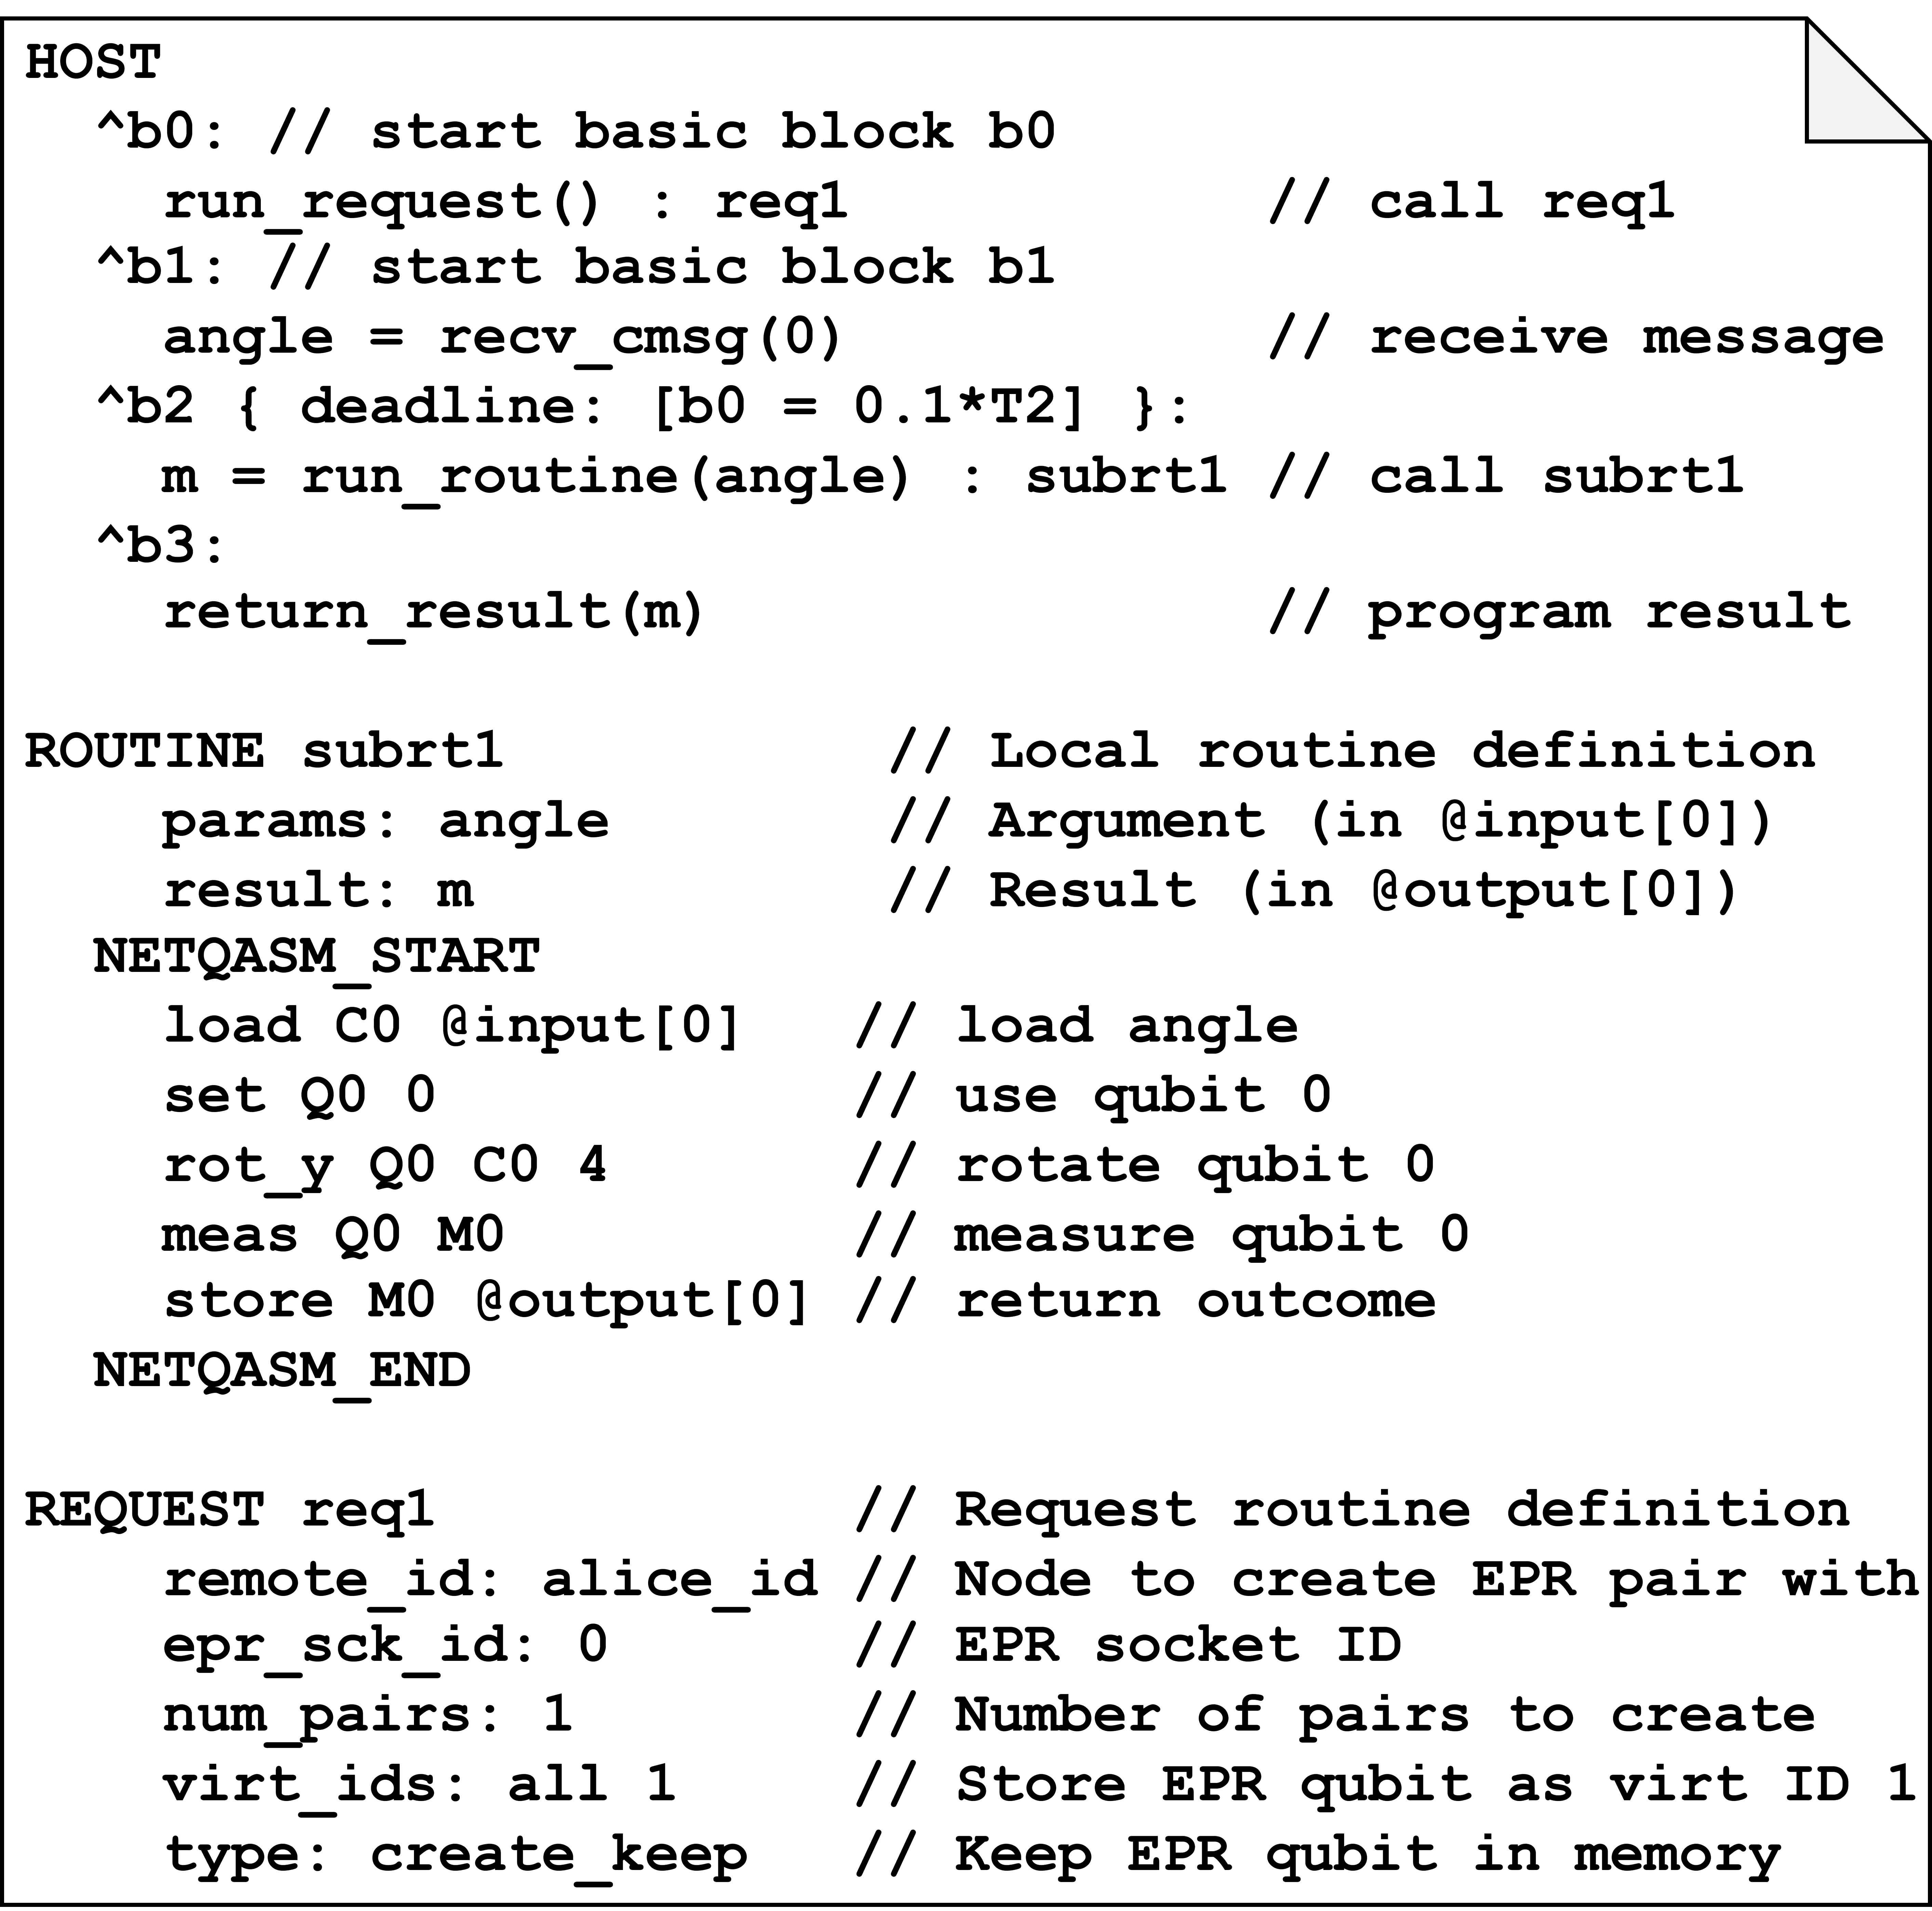
\includegraphics[width=\columnwidth]{figures/qoala/example_program.png}
    \caption{
        Example Qoala program containing a host section with 4 blocks, a local routine (\texttt{subrt1}),
        and a request routine (\texttt{req1}). Block \texttt{b2} has a relative deadline to \texttt{b0} of $0.1$ times qubit noise parameter $T_2$.
    }
    \label{fig:example_program}
\end{figure}

\begin{figure*}
    \newcommand{\figheight}{6.5cm}
    \centering
    \subfloat[\centering \label{fig:task_types}]{{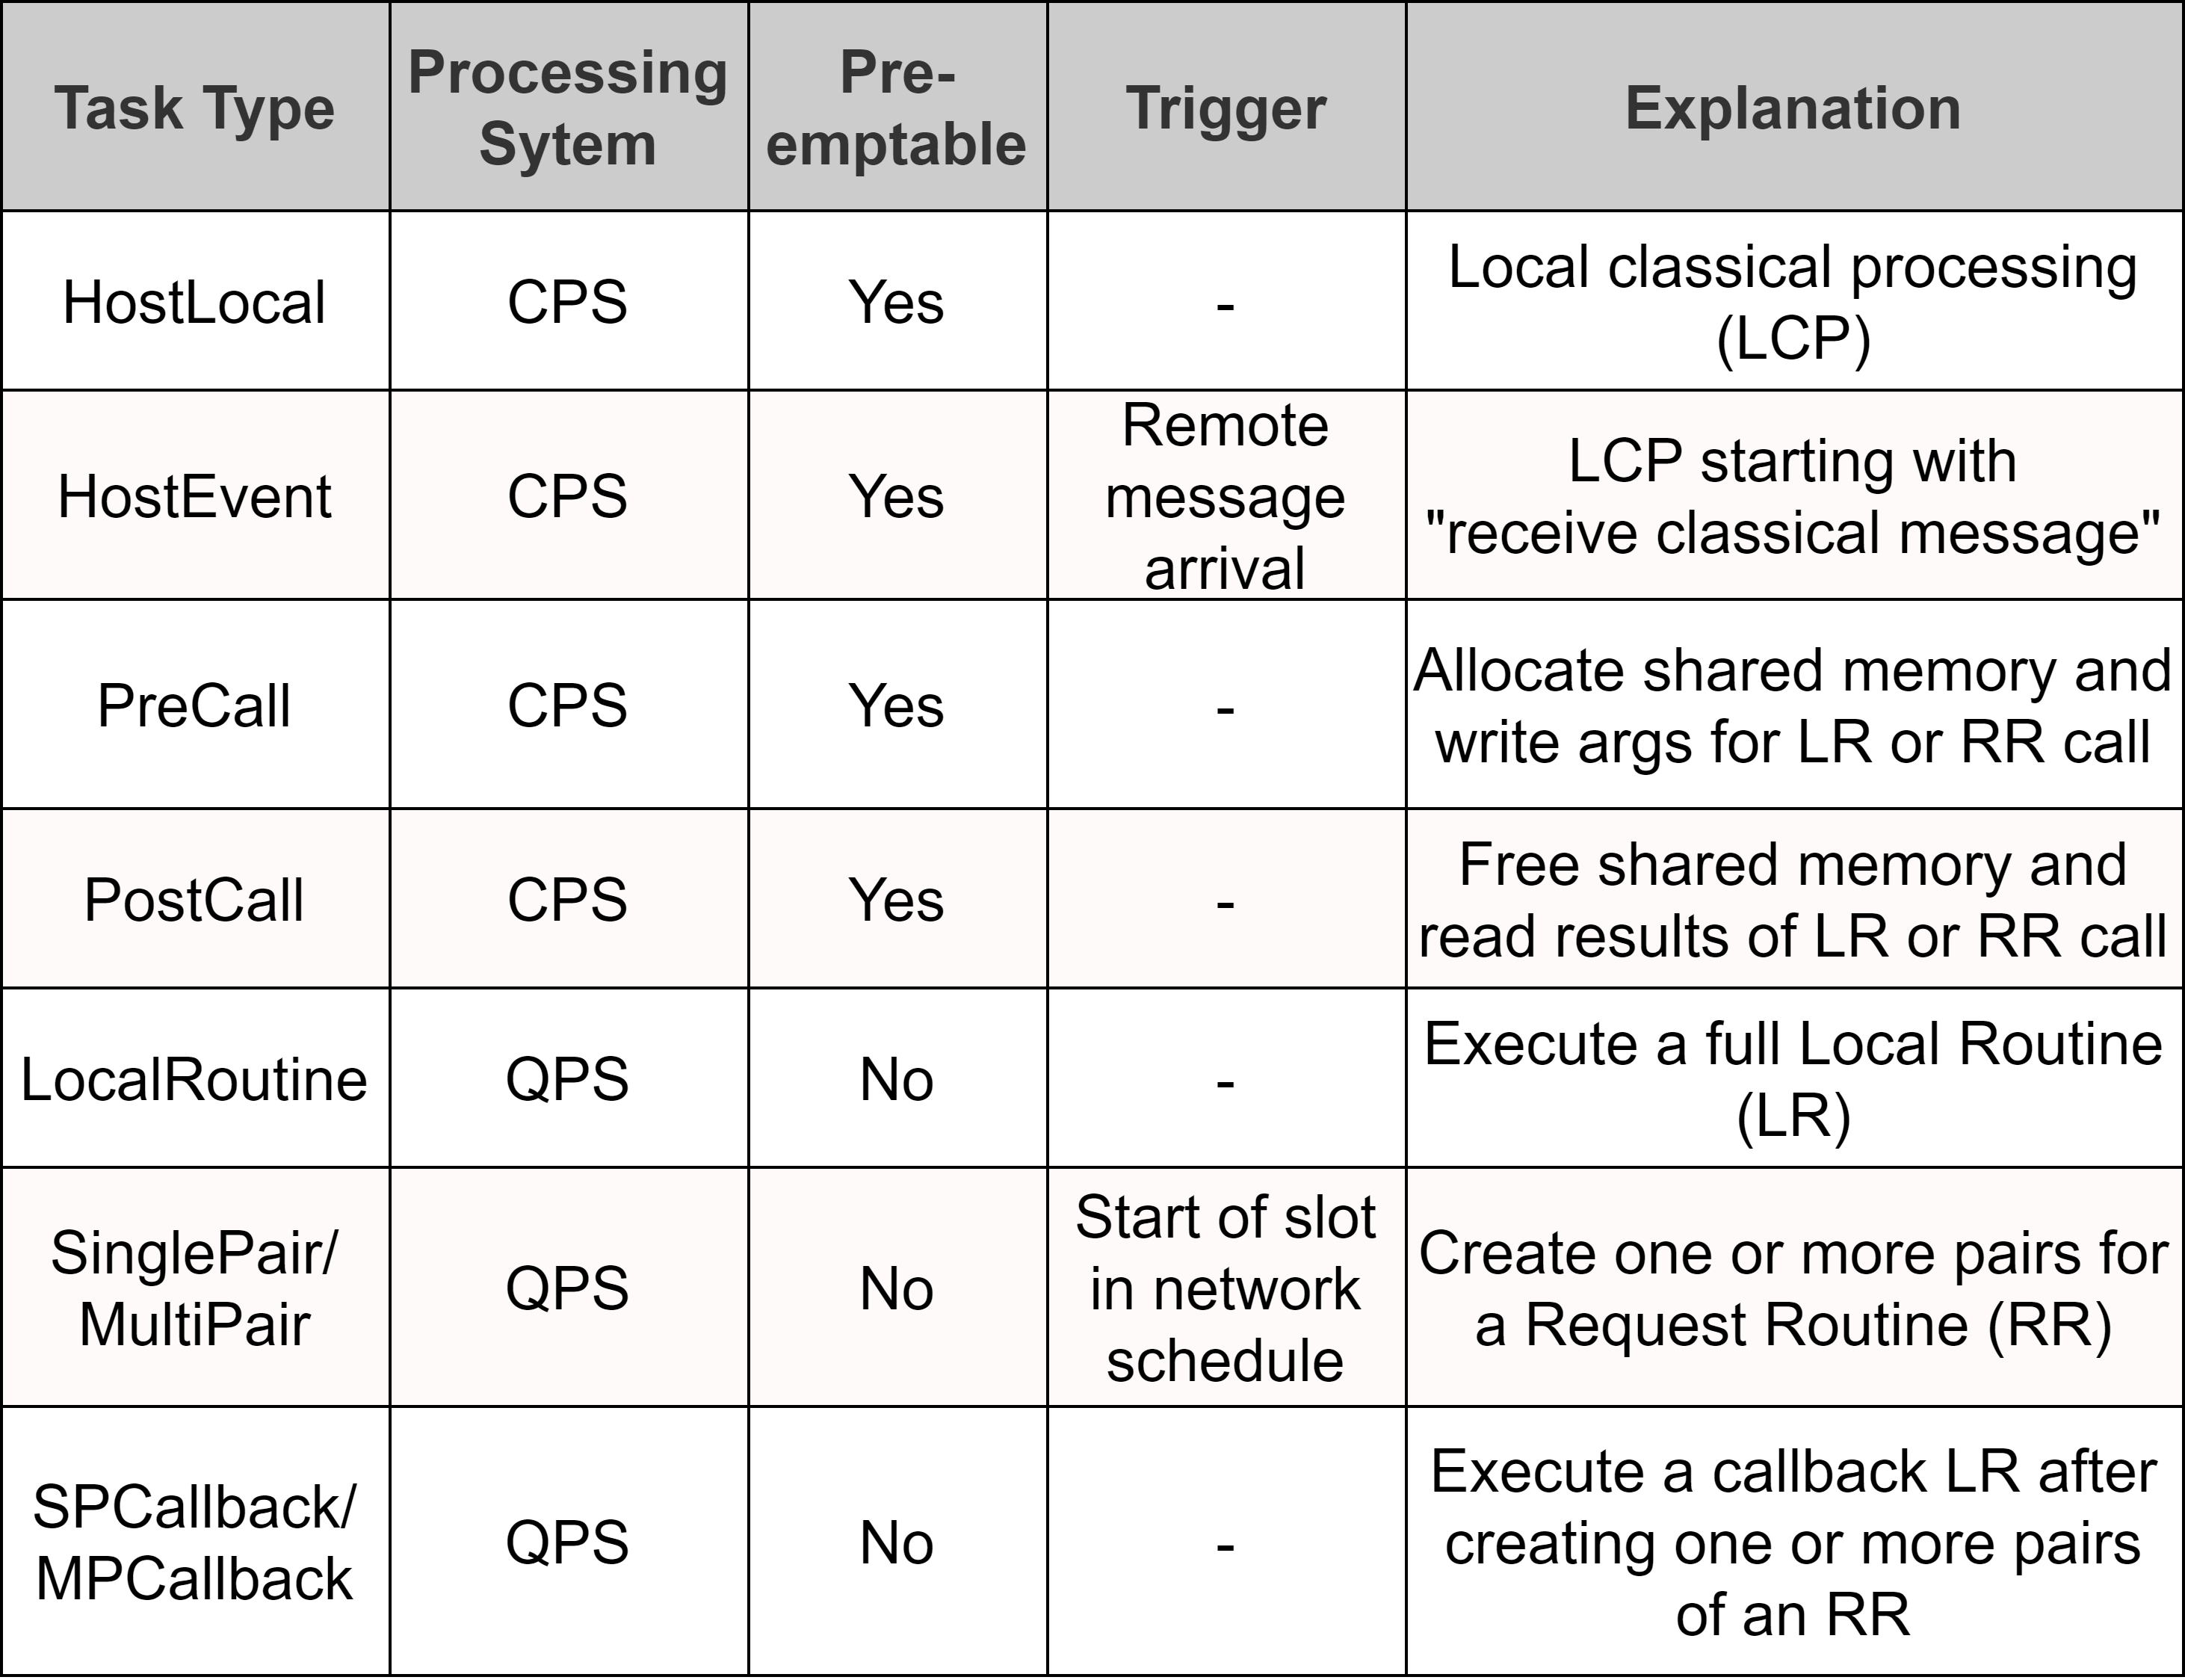
\includegraphics[height=\figheight, keepaspectratio]{figures/qoala/task-types-table.png}}}%
    \hfill
    \subfloat[\centering \label{fig:task_creation_cutout}]{{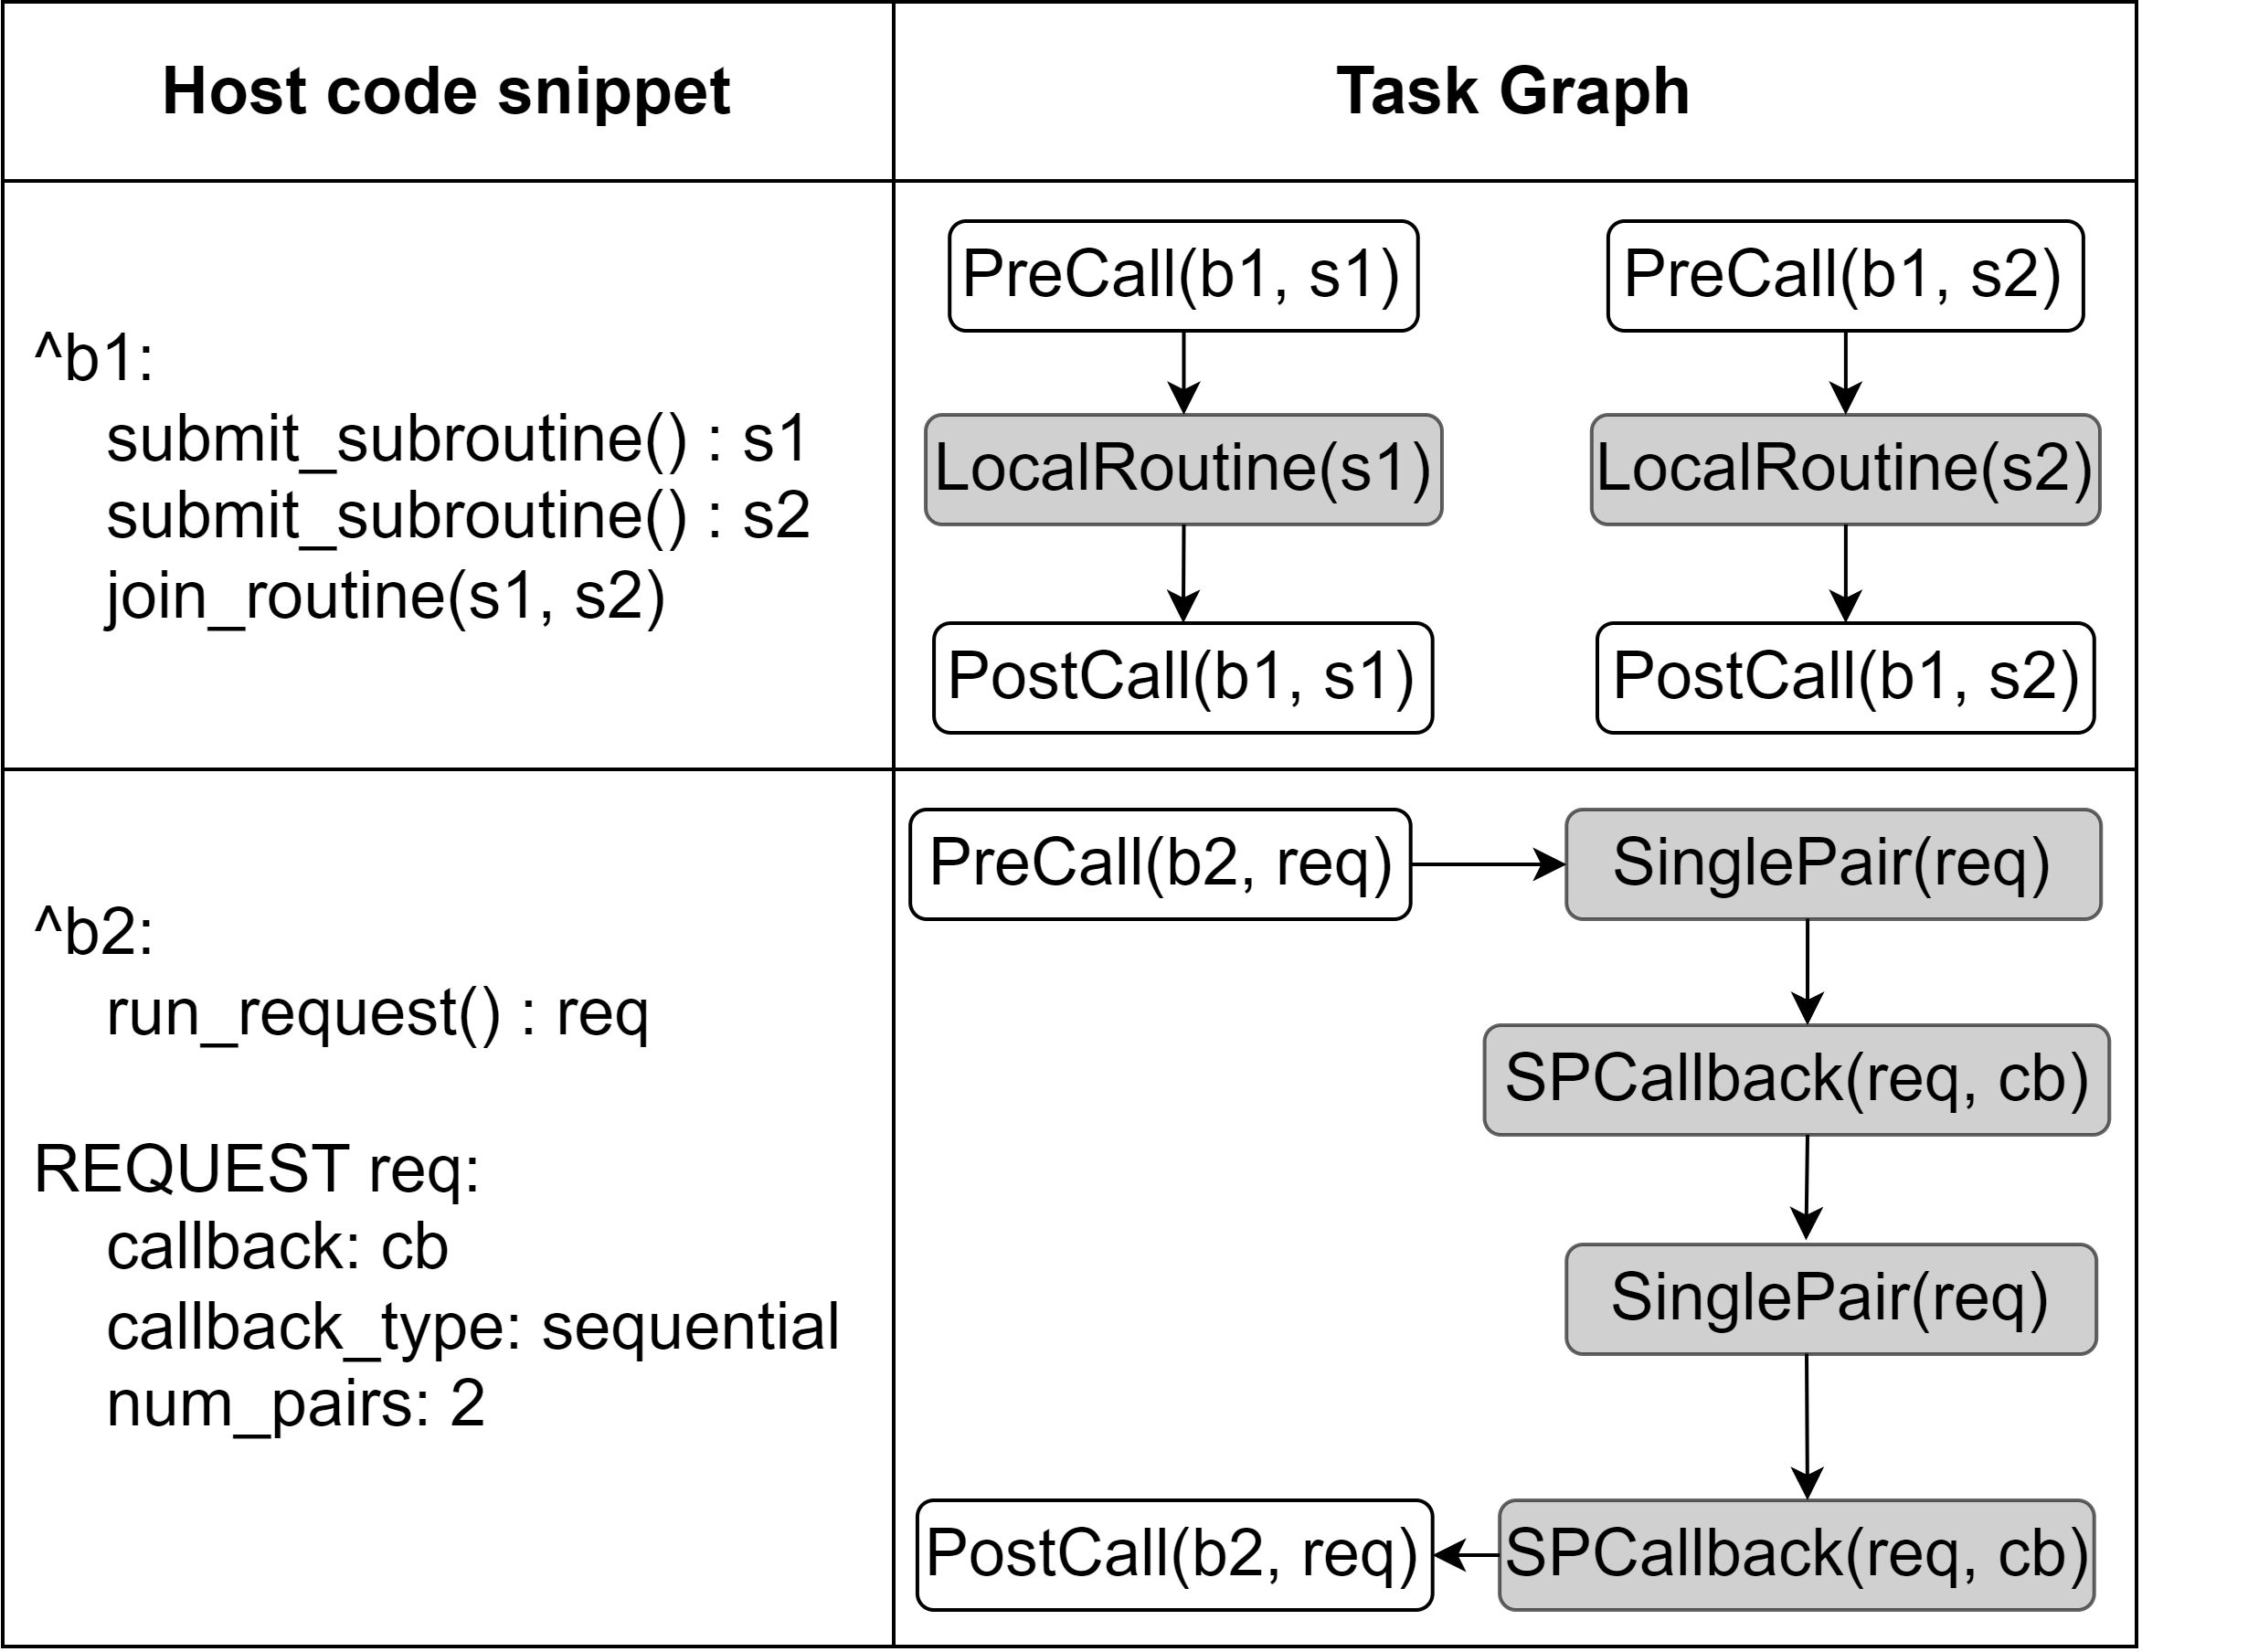
\includegraphics[height=\figheight, keepaspectratio]{figures/qoala/task_creation_cutout.png}}}%
    \caption{
        (a) Overview of task types.
        (b) Examples of host code and corresponding task graphs.
        Shaded tasks are executed by the QPS, the others by CPS.
        Top: asynchronous submission of local routines \texttt{s1} and \texttt{s2}.
        The graph consists of two separate chains of tasks and the scheduler can choose in which order to execute these chains (possibly interleaved).
        Bottom: a request routine uses the callback entry to immediately add tasks for executing local routine \texttt{cb} after each entangled pair generation.
    }%
    \label{fig:tasks}
\end{figure*}

\subsection{Tasks}
\label{qoala:sec:tasks}
We introduce \textit{tasks} to enable multitasking.
Each task represents a code segment of a running program with a context of runtime variables.
Tasks have different types (Figure~\ref{fig:tasks}) based on the code they represent.
By splitting a program into distinct executable tasks, 
we can utilize the parallel execution on the CPS and QPS (by assigning tasks to the corresponding system),
and we can interleave execution of multiple programs by filling waiting times of one program by execution of tasks of another.
Code segments indicated to run asynchronously (Section~\ref{qoala:sec:program_structure}) can also be represented by tasks, the execution order of which can then be governed by a scheduler.
%, simplifying the interface between the developer's intent (`run these segments in any order') and the runtime system (choosing an efficient execution order).
Further, tasks enable interleaving of local operations and quantum network (entanglement generation) operations.
A scheduler can choose when to execute entanglement tasks (with strict timing requirements from the network schedule)
and when to execute local tasks (less strict requirements).

\textit{Task graph}.
Tasks are organized in a \textit{task graph}, a directed acyclic graph (DAG) where each node represents a single task.
Edges can be \textit{precedence constraints} (task A must conclude before task B initiates) or \textit{relative deadlines} (task B should start within maximum duration $t$ after completion of task A).
Using a task graph introduces a well-defined and isolated scheduling problem: given a graph of tasks, which task(s) should be executed next?
Deadlines are used to assist the scheduler (see below) in mitigating the gradual quality degradation of quantum states over time (decoherence) by choosing appropriate tasks.
Some tasks are only enabled after certain events happen.
\texttt{HostEvent} tasks are enabled by an incoming classical message and \texttt{SinglePair} or \texttt{MultiPair} tasks are enabled by network schedule timestamps.
Tasks also have information about what quantum memory they use, helping the scheduler decide which tasks it can execute at a given time.

\textit{Task creation}. 
A task is created for a segment of a running program.
If a program segment is executed multiple times (e.g. because of a loop in the code), this results in multiple tasks.
A host code block is translated into a \texttt{HostLocal} task (block contains only local instructions) or a \texttt{HostEvent} task (block starts with a `receive message' instruction).
A local routine call is represented by (1) a \texttt{PreCall} task (CPS allocates shared memory and writes routine arguments), (2) a \texttt{LocalRoutine} task (QPS executes routine), and (3) a \texttt{PostCall} task (CPS reads routine results from shared memory).
Request routine calls are handled similarly (with \texttt{SinglePair} or \texttt{MultiPair}).
\texttt{MultiPair} tasks can be more time- and resource efficient since the network stack can handle multiple pair generations at once.
Callback tasks for local routines acting as entanglement generation callbacks allow quick successive execution.
For each task, its expected duration is calculated based on the metadata of the corresponding block or routine in the program, together with information from the EHI (see below).
See Figure~\ref{fig:task_types} for task types and Figure~\ref{fig:task_creation_cutout} for examples of host code and corresponding tasks (details in Appendix~\ref{qoala:sec:app:scheduling_execution}).


\subsection{Program instantiation}
\label{qoala:sec:program_instantiation}
A program is part of an application that uses entanglement generation orchestrated by a network controller (Figure~\ref{fig:program_illustration}).
Therefore, before execution, the program must align with the other programs of its application as well as with the network controller.
(1) \textit{Capability negotiation and entanglement demand registration}.
First, all collaborating nodes exchange their EHI and agree on concrete values for deadlines and task duration estimations (using advice pre-computed by the compiler).
These values are needed to do effective scheduling at runtime.
Second, the nodes together register their entanglement demands to the network controller, which then creates a \textit{network schedule} based on these.
This schedule consists of time slots, each of which is assigned to an individual \textit{application instance} (tuple of program instances, one per node).
(2) \textit{Program instantiation}. Concrete values for program arguments can be filled in such as deadlines, durations and program-specific input values.
Typically, for a given application, the involved nodes create many \textit{program instances} of the same program (to gather statistics, Section~\ref{qoala:sec:background_context}).


\subsection{Scheduling and execution}
\label{qoala:sec:scheduling}
Tasks produced for program instances are executed by the \textit{node scheduler}.
This scheduler manages a global task graph containing all tasks that have been created for instantiated programs and that are awaiting execution
Among the tasks that do not have any precedence constraints going into them (anymore), the scheduler continuously chooses the next task(s) to execute.
It may choose to run a task on the CPS and a task on the QPS in parallel.
If a task completed successfully, it is removed from the task graph, and precedence constraints and relative deadlines are updated accordingly.
Based on the control flow of the program that this task was for, new tasks may be created representing the next segment of the program.
These tasks are then added to the task graph.
If a task failed (for example, entanglement generation did not succeed for a \texttt{SinglePair} task), it either (a) remains in the task graph and may be scheduled again at a later time,
or (b) the whole program instance is aborted, depending on the scheduler implementation.
For \textit{predictable programs} (where control-flow and hence all corresponding tasks are known beforehand), their entire task graph may be created ahead of execution
and (no need to add new tasks at runtime).
Tasks for entanglement generation (like \texttt{SinglePair}) additionally contain information about when they are allowed to start according to the network schedule,
allowing the scheduler to make sure that the network schedule is respected.
The scheduler allows pre-emption of CPS tasks.
For instance, the arrival of a message from a remote node might activate a \texttt{HostEvent} task with high priority;
if the CPS was executing another lower priority task, it may be pre-empted and resumed at a later time.
Since quantum tasks cannot in general be rolled back or resumed (e.g. measurements are destructive and cannot be undone), Qoala does not allow the pre-emption of QPS tasks.
Although we define a scheduling problem, and a framework for designing and implementing scheduling algorithms,
we on purpose do not prescribe an explicit implementation and leave the question of an optimal scheduling approach open for further research (Section~\ref{qoala:sec:conclusion}).

\section{Implementation}
\label{sec:implementation}
We implement our architecture in the form of an open-source simulator~\cite{qoala2023simulator}.
Implementation on real hardware requires developing new classical control hardware which is outside the scope of this work.
The simulator is built on top of NetSquid~\cite{coopmans2021netsquid} which can simulate quantum behavior as well as asynchronous classical processes.
Specifically, NetSquid provides detailed configuration allowing for simulations of hardware with parameters that are validated in real experiments, not possible using other simulators such as QuNetSim~\cite{diadamo2021qunetsim}, QNET~\cite{QNET}, and QuISP~\cite{satoh2022quisp}.
SquidASM~\cite{squidasmrepo} simulates the software and hardware stack used in the NetQASM/QNodeOS system mentioned in Section~\ref{sec:related_work}, and hence misses the scheduling capabilities that we introduce in Qoala.

The simulator has on purpose been made modular and composable:
components of Qoala's architecture (like CPS, QPS, scheduler, shared memory) are provided by the simulator as building blocks that can be configured and put together in different ways (details Appendix~\ref{sec:app:simulator}).
Both classical software parameters and quantum hardware noise models can be configured.
In this way, the simulator allows one to investigate different architecture and parameter choices.
% , and can therefore be used beyond just testing the Qoala architecture.
In the simulator, a network of quantum nodes implementing Qoala can be constructed, and Qoala programs can be submitted for execution to these nodes.
Static network schedules can be provided (capability negotiation and automatic network schedule creation are not simulated).
The simulator then executes the programs, providing application results and statistics.
% The simulator has also been used to perform our evaluation.
Our implementation allows researchers to not only test Qoala, but also configure parameters and architectures to investigate scheduling algorithms and hardware implementation choices.

\subsection{Scheduler implementation}
In our implementation, we use a two-level hierarchical scheduler architecture,
consisting of a node-wide \textit{node scheduler} which controls two \textit{processor schedulers}, one for the CPS and one for the QPS (Figure~\ref{fig:scheduler_impl}, details in Appendix~\ref{sec:app:scheduling_execution}).
Such an approach has been used in other contexts not related to quantum networks~\cite{polychronopoulos1991hierarchical, girkar1994hierarchical}.

Each scheduler maintains their own task graph.
The node scheduler task graph contains all tasks (CPS or QPS) that are to be executed.
Each processor scheduler task graph is a partial copy of the node scheduler task graph containing only the tasks that can be executed by its own processor.
Edges in the node scheduler graph between heterogeneous tasks (i.e. between CPS and QPS tasks) are represented in the partial processor graphs by an \texttt{external-dependencies} node attribute. 
When a processor scheduler finishes a task, it is removed from the task graph and a signal is sent to the node scheduler.
The node scheduler updates its own task graph accordingly, and may then add new tasks to the task graph of the processor scheduler.
Write conflicts on the processor task graphs are avoided since tasks can only be added by the node scheduler, and tasks can only be removed by the processor scheduler.

The processor schedulers support both a first-come-first-serve (FCFS) and an earliest-deadline-first (EDF)~\cite{silberschatz2006operating} scheduling mechanism.
In our evaluation (Section~\ref{sec:evaluation}), deadlines are used as \textit{soft deadlines}, i.e. there is no guarantee about meeting deadlines.

\begin{figure}% [ht]
    \centering
    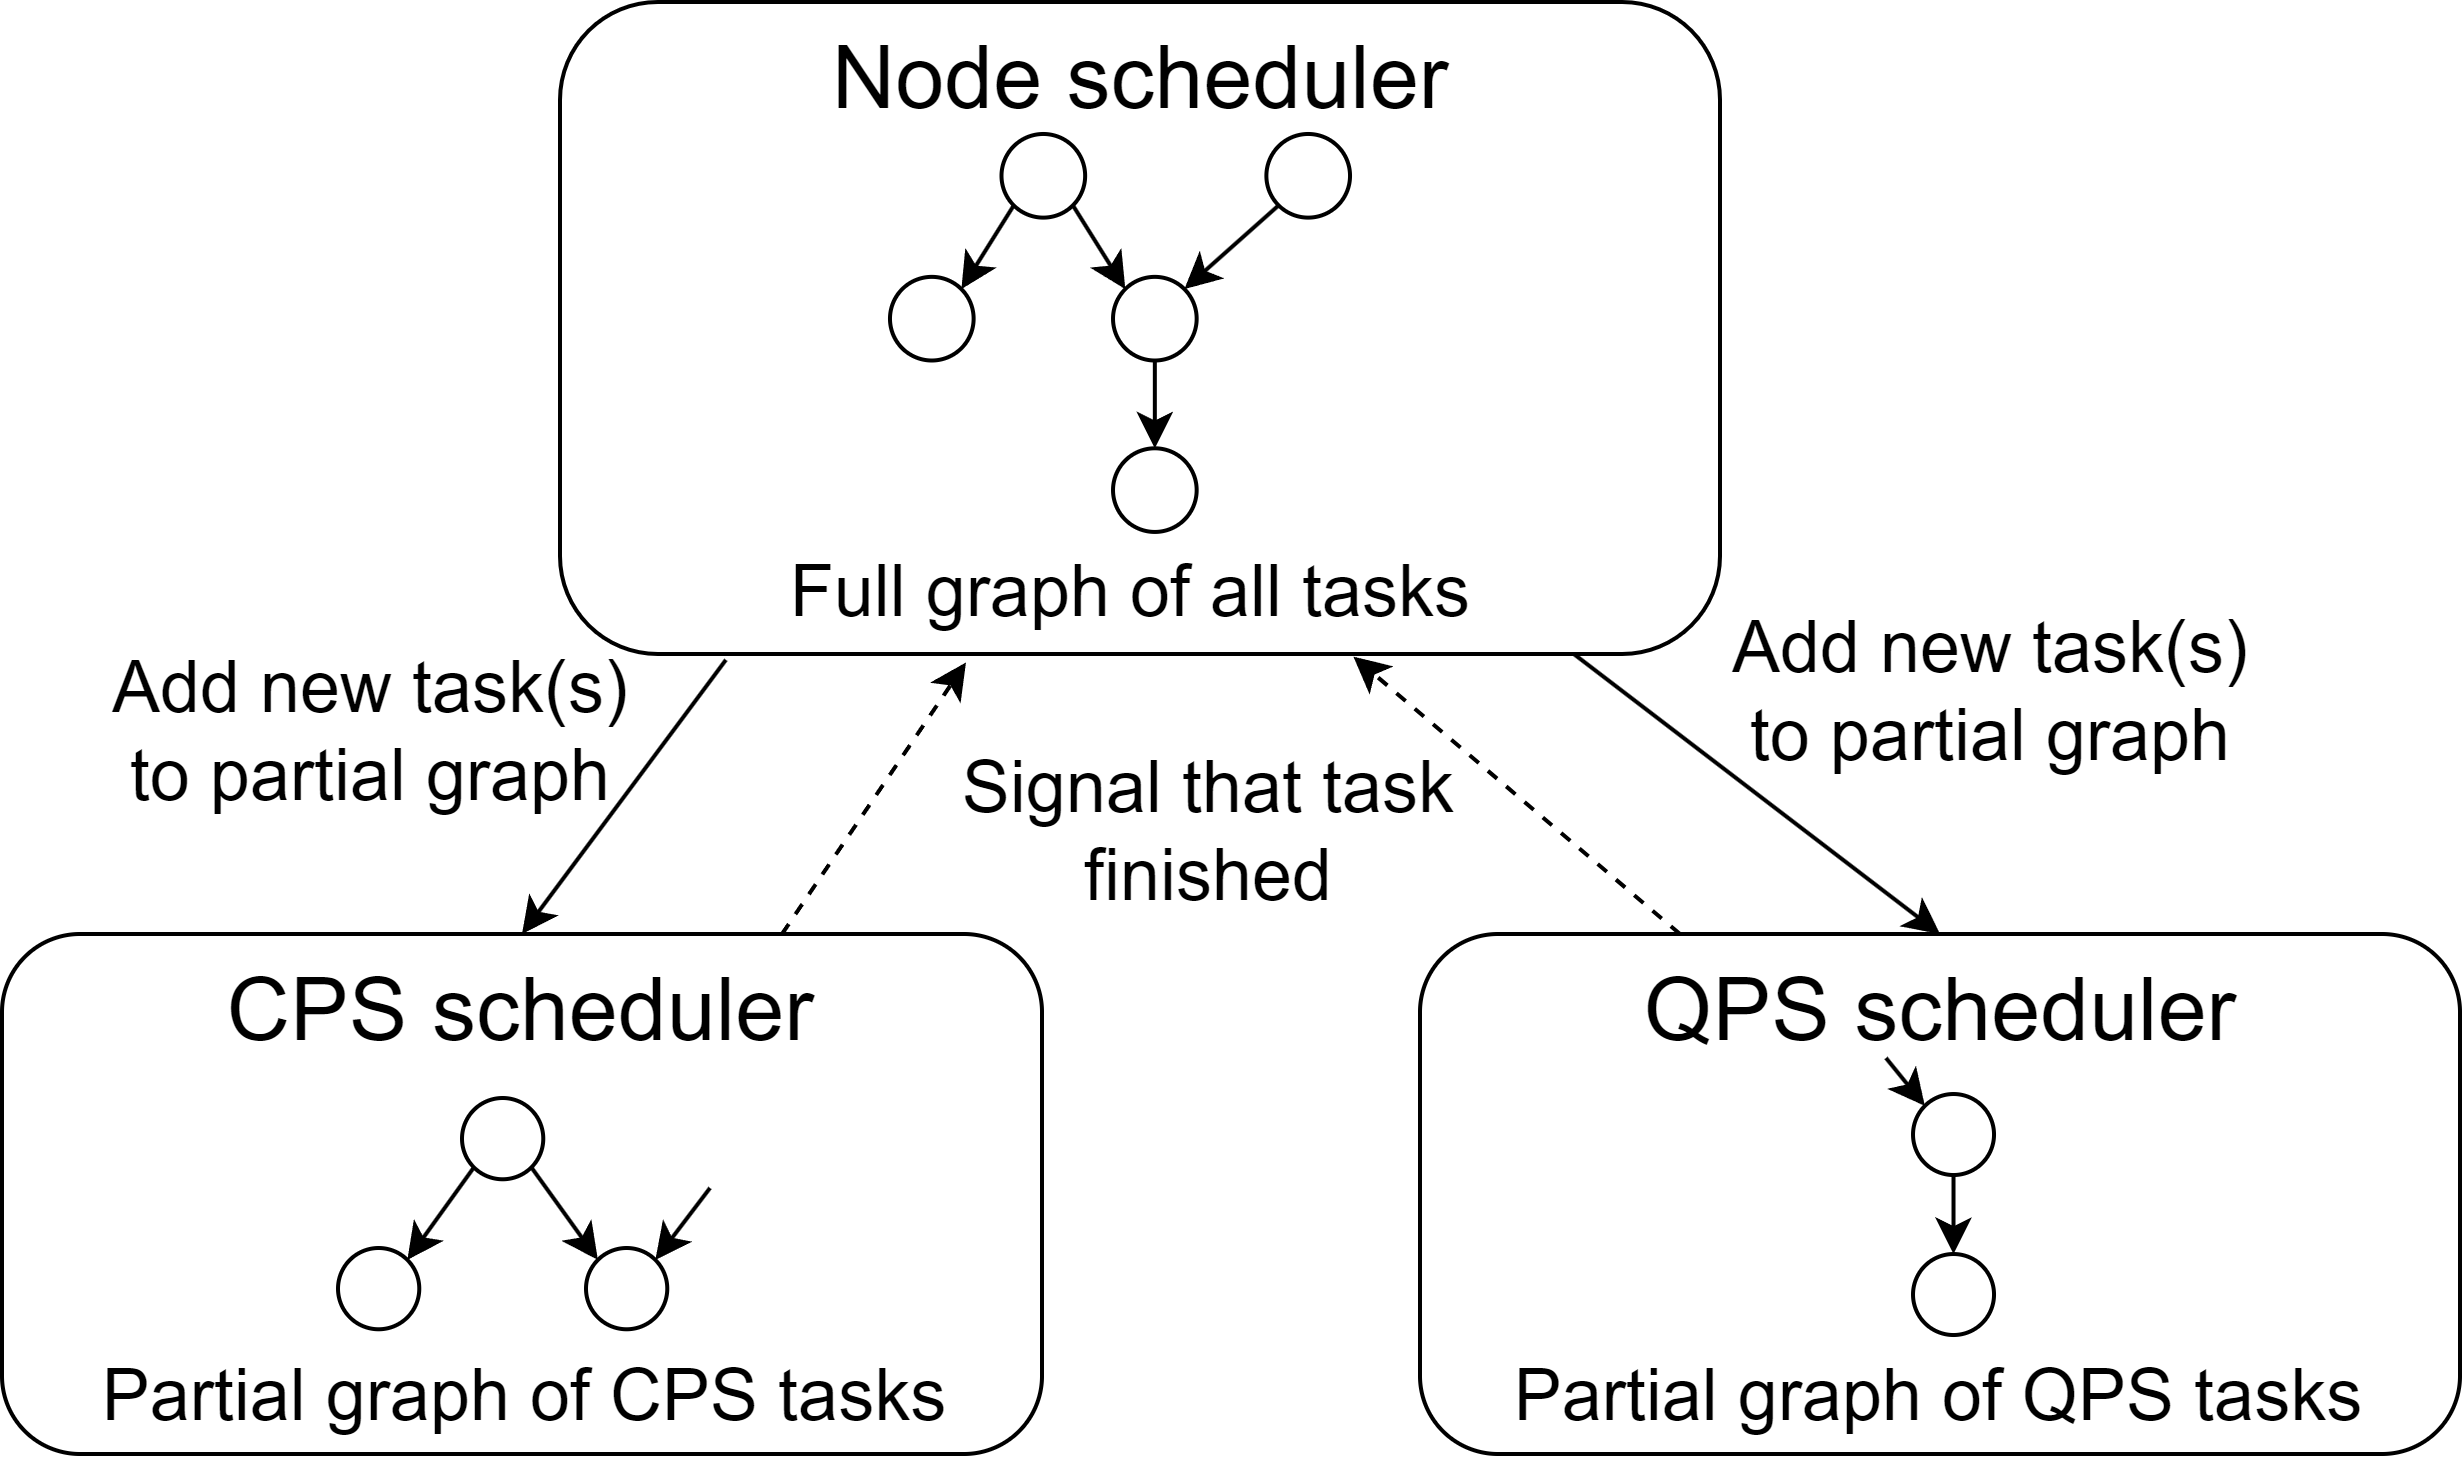
\includegraphics[width=\columnwidth]{figures/qoala/scheduler_components.png}
    \caption{Overview of our hierarchical scheduler implementation.
    The node scheduler maintains a graph of all tasks. The CPS and QPS maintain partial graphs with only tasks they can execute themselves. Partial graphs are updated by the node scheduler. 
    The CPS scheduler has access to a buffer with classical messages from other nodes, activating \texttt{HostEvent} tasks. The QPS scheduler has access to the network schedule, determining allowed start times of \texttt{Pair} tasks.}
    \label{fig:scheduler_impl}
\end{figure}





\section{Evaluation}
\label{sec:evaluation}
All simulations were run on a machine using 80 Intel Xeon Gold cores at 3.9 GHz and 192 GB of RAM.
Each subsection describes an independent evaluation (details in Appendix \ref{sec:app:evaluation}):

\subsection{Demonstrating the architecture's effectiveness}
\label{sec:demonstrating_architecture_effectiveness}
We first validate the functionality of our architecture by demonstrating that applications of different CPS-QPS interactions types can successfully be executed on two or more nodes.
Using our implementation (Section~\ref{sec:implementation}), we report that we successfully simulated the following applications:
(A1) quantum key distribution (2 nodes, first QPS generating $10^3$ EPR pairs followed by only CPS actions (classical computation and messaging)),
(A2) blind quantum computation (1 client and 1 server node, first QPS generating 2 EPR pairs, then CPS performing rounds of classical messaging followed by local quantum gates by QPS),
(A3) single-qubit teleportation across two nodes (1 sender and 1 receiver node, QPS generating one EPR pair followed by QPS measurement by the sender, CPS classical messaging and QPS local quantum gates by the receiver),
(A4) a ping-pong application which repeats the single-qubit teleportation application to transfer states back and forth,
and (A5) a multi-node GHZ-state~\cite{greenberger1989going} creation application (3 nodes, QPS creating a tripartite entangled state using multiple EPR pairs, using CPS classical messaging and QPS local quantum gates).

Each program is instantiated 1000 times and all tasks are immediately added to the task graph (since the the programs are \textit{predictable} (Section~\ref{sec:scheduling})).
Precedence constraints are added such that instances are executed sequentially for simplicity.
We use a fixed network schedule (no demand registration (Section~\ref{sec:program_instantiation}) since network schedule generation is not handled by Qoala itself and hence not part of the evaluation).
To demonstrate the hardware independent performance of Qoala, all simulations are performed on three different hardware models: a generic quantum platform (uniform qubit connectivity and \textit{vanilla} NetQASM instruction set~\cite{dahlberg2022netqasm}),
and two models based on data validated on real hardware (NV centers~\cite{bradley2019ten, hermans2022qubit} and trapped ions~\cite{krutyanskiy2023entanglement}). 
We observe successful execution (desired deterministic outcome when setting noise parameters (Section~\ref{sec:background_context}) to 0, and expected non-deterministic outcome distributions with realistic noise parameters) for all types of applications (details in Appendix~\ref{sec:app:evaluation}).

\begin{figure}% [ht]
    \centering
    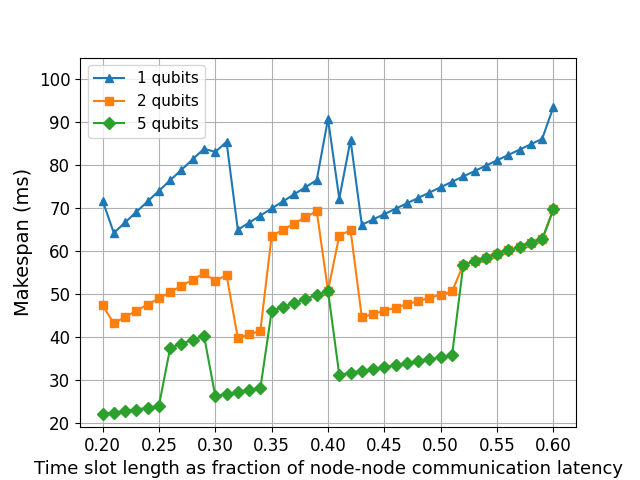
\includegraphics[width=1.0\columnwidth]{figures/teleport-self-preemption.png}
    \caption{Self-preemption of a teleportation program.
    For certain durations of the time slot length (as fraction of node-node communication latency, x-axis), the makespan is considerably higher (spikes in the plot).
    Reason: a classical message arrives for some teleportation instance $i$,
    making the node scheduler choose to perform the local quantum gates for $i$. During this,
    the time slot for instance $j > i$ starts. Since the QPS is busy with $i$, it cannot work on entanglement
    generation for $j$. Therefore, $j$ must wait for the next repetition of the network schedule, leading to a higher overall makespan.
    }
    \label{fig:teleport_self_preemption}
\end{figure}

\subsection{Demonstrating Qoala's multitasking potential}
Next, we demonstrate that Qoala can execute multiple instances of (different) programs concurrently by interleaving. We examine (1) makespan decrease (Section~\ref{sec:background_context}) when interleaving the instances compared to sequential execution, % (scheduling all instances in sequence).
(2) whether makespan depends on the network schedule.

We first evaluate multitasking instances of the same application: teleportation (same as A3 in \ref{sec:demonstrating_architecture_effectiveness}), 100 instances, with a fixed network schedule (no time slots; entanglement generation always allowed).
Sequential scheduling of instances results in makespan $N \cdot CC$
while interleaved scheduling (tasks for all instances created at the same time; no precedence constraints between instances) results in $\left\lceil N / Q \right\rceil \cdot CC$
(number of instances $N$, classical node-node communication latency $CC$, number of available memory qubits at receiving node $Q$).
We also evaluate the effect of network schedules with time slots (repeating pattern of slots assigned to A3 instances), and find that the time slots length influences the makespan (Figure~\ref{fig:teleport_self_preemption}) in a non-trivial manner due to instances pre-empting each other.
BQC (same as A2 in \ref{sec:demonstrating_architecture_effectiveness}, 100 instances) interleaved gives a makespan decrease over sequential of ($21\%, 56\%, 65\%$) for (2, 5, 10) server qubits, respectively.
The network schedule affects the makespan decrease: doubling the time slot length results in a smaller decrease ($12\%, 48\%, 48\%$). 

We then execute instances of different applications and again examine the effect of the network schedule on the makespan decrease: 50 QKD (A1 in \ref{sec:demonstrating_architecture_effectiveness}) and 50 BQC (A2) instances give a makespan decrease of $9.5\%$ (fixed schedule which first has time slots for QKD and then for BQC) and $39\%$ (schedule with time slots alternating between QKD and BQC).
We observe that multitasking can lead to improved (lower) makespan and that the network schedule can have considerable impact on the makespan.

\begin{figure}% [ht]
    \centering
    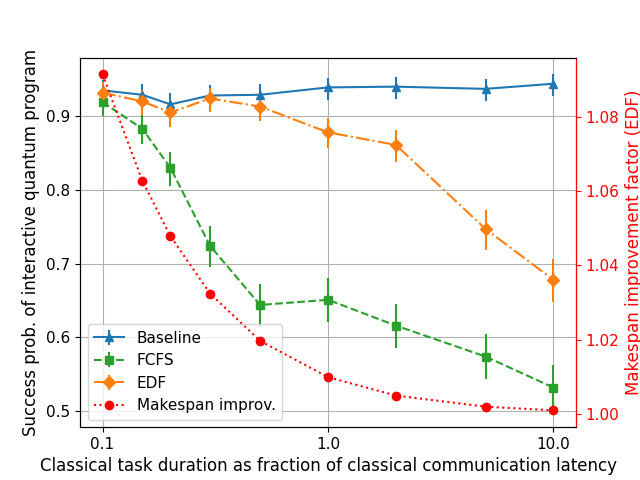
\includegraphics[width=1.0\columnwidth]{figures/tradeoffs_cq.png}
    \caption{Execution of interactive quantum program in the presence of a `busy' CPS program (tasks with duration $f \cdot CC$ for fraction $f$ of the classical node-to-node latency $CC$, x-axis).
    \textbf{Comparison of schedulers:}
    $Baseline$ (no scheduling nor interleaving),
    $FCFS$: first-come-first-serve scheduler (interleaving possible, no deadlines to prioritize quantum tasks),
    $EDF$: earliest-deadline-first scheduler (with deadlines to prioritize quantum tasks).
    The interactive program regularly waits (duration $CC$), with quantum states in memory, for incoming classical messages. % before continuing.
    Task interleaving allows busy CPS tasks to fill waiting times.
    EDF leads to higher success probability than FCFS, showcasing usefulness of deadlines.
    \textbf{Tradeoffs:}
    The baseline of sequential execution leads to the best possible success probability (quantum metric) at the expense of longest makespan. EDF allows a lowering of makespan (classical metric) at the expense of a lower succ. prob. (quantum metric). 
    % leads to the best succ. prob. since there is no interleaving (while qubits are in memory).
    %EDF succ. prob. lower than baseline is juxtaposed by an improvement (decrease) of makespan (improvement factor above 1, plotted on right axis as baseline makespan divided by EDF makespan).
    }
    \label{fig:eval_tradeoffs_cq}
\end{figure}

\subsection{Improvement over NetQASM architecture}
\label{sec:improvement_over_netqasm}
We compare the Qoala architecture with the NetQASM runtime approach for executing programs on a node from~\cite{dahlberg2022netqasm}
and show that Qoala provides new compilation possibilities (optimizing across classical and quantum code) and can lead to a better application execution makespan.
We consider a remote measurement-based quantum computing program written in Python (the program format of the NetQASM runtime) which has suboptimal code logic on purpose.
Executing this program in the NetQASM runtime performs worse (success probability $66\%$) than the same program but compiled manually into a Qoala program and executed in the Qoala runtime (succ. prob. $82\%$).
We note that manual compilation allowed optimization that is not possible in the NetQASM program format, exemplifying the new compilation potential provided by Qoala.

\begin{figure*}
    \newcommand{\heatmapheight}{6.6cm}
    \centering
    \subfloat[\centering \label{fig:heatmap_teleport}]{{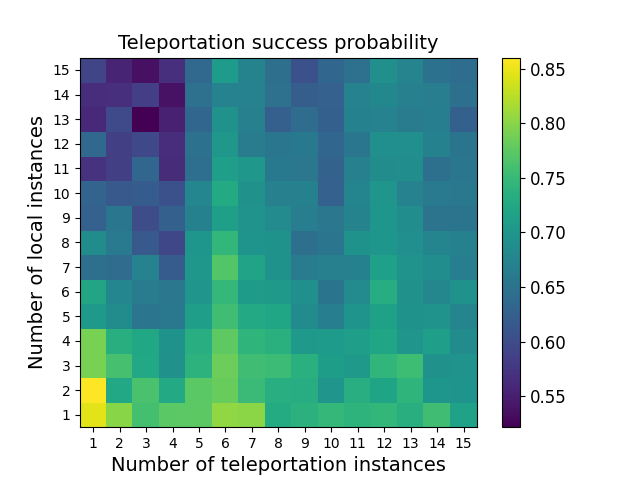
\includegraphics[height=\heatmapheight, keepaspectratio]{figures/heatmap_teleport.png}}}%
    \hfill
    \subfloat[\centering \label{fig:heatmap_local}]{{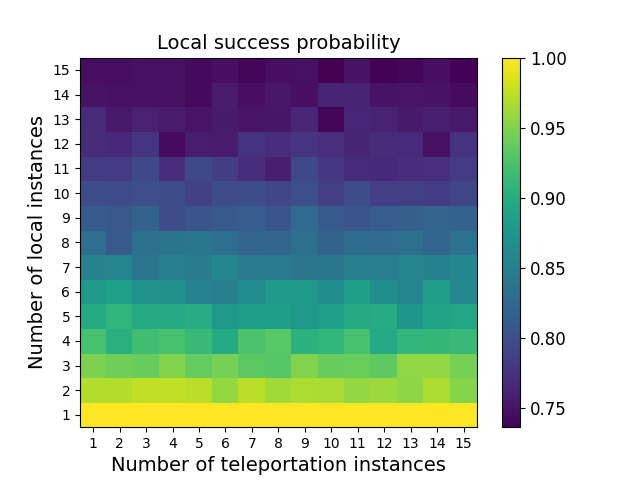
\includegraphics[height=\heatmapheight, keepaspectratio]{figures/heatmap_local.png}}}%
    \caption{
        Concurrent execution of teleportation (A3) and a local application (only preparing and measuring qubits).
        (a) Success probability of teleportation for different numbers of teleportation and local instances.
        More local instances lead to lower teleportation succ. prob. (effect more pronounced with few teleportation instances).
        (b) Success probability of local program. More local instances lead to lower local succ. prob., independent of the number of teleportation instances.}%
    \label{fig:quantum_multi_tasking}%
\end{figure*}


\subsection{Tradeoffs between classical and quantum performance metrics}
\label{sec:effectiveness_of_task_splitting}
We compare different scheduling modes enabled by Qoala and evaluate tradeoffs between makespan and success probability, noting that the NetQASM runtime did not allow scheduling at all (Figure~\ref{fig:eval_tradeoffs_cq}).
We expect that interleaving of tasks reduces the makespan, but may lead to lower success probability due qubits degrading in memory while tasks wait for each other.
We compare 3 scheduling modes: no scheduling (baseline), FCFS scheduling, and EDF scheduling.
We consider a simple runtime scenario with 
(1) a local quantum program which alternates between doing local quantum gates and waiting for a remote classical message before continuing and 
(2) a classical `busy program' consisting only of CPS tasks (duration defined as fraction of classical node-node latency).
We find that
(a) scheduling (FCFS or EDF) decreases success probability (EDF less than FCFS); impact larger for long task durations, but
(b) EDF provides a better makespan than no scheduling.
Note that the baseline necessarily gives the highest success probability due to no waiting, but at the expense of maximal makespan (sequential execution).

\subsection{Success probabilities with quantum multitasking}
\label{sec:quantum_multitasking}
Next, we consider a quantum multitasking scenario where we investigate trends in application success probability while varying the number of concurrent applications (Figure~\ref{fig:quantum_multi_tasking}).
In addition to a teleportation application (A3 in \ref{sec:demonstrating_architecture_effectiveness}), the receiver node also executes multiple instances of a local quantum program (only applying quantum gates).
Whenever the receiver node must wait for classical messages to come in for A3, it can work on its local quantum programs.
We find that success probability of both types of programs decreases in the presence of another program.

\subsection{Performance sensitivity}
Finally, we investigate the influence of classical message-passing latencies, internal latencies, and network schedule contents on application success probability of BQC (A2, 100 instances).
We find that the duration of sending classical messages between nodes has a large impact on the success probability:
node-node latencies [$0.01$, $0.1$, $1$] times the qubit coherence time lead to success probabilities [$0.89(2)$, $0.83(2)$, $0.54(4)$], respectively.
Internal latencies (between CPS and QPS, and between the scheduler and CPS or QPS) only have a significant impact when message-passing durations are low (0.01 times the qubit coherence time).
We also compare different network schedules (simple linear repeating schedule where each client-server pair gets a time slot consecutively; slot length is varied).
We obtain success probabilities [$0.90(2)$, $0.69(3)$, $0.48(4)$] for time slot lengths [$0.01$, $0.1$, $1$] times the qubit coherence time, respectively.

\section{Conclusion}
\label{qoala:sec:conclusion}
Qoala is the first architecture for executing quantum applications that addresses the need for scheduling and compiling hybrid classical-quantum programs for a quantum internet.
This allows Qoala to ensure successful execution of quantum programs even in the presence of limited quantum memory lifetimes, and opens the door for a compile time optimization of the hybrid classical-quantum program.
By building on an existing quantum network stack~\cite{dahlberg2019link, pompili2022experimental} and the implementation of QNodeOS on quantum hardware~\cite{pompili2022experimental, carlothesis} we pave the way for the real-world implementation of Qoala in a platform-independent way on diverse hardware platforms including NV centers in diamond~\cite{pompili2021realization, pompili2022experimental}, or Ion Trap~\cite{krutyanskiy2023entanglement,krutyanskiy2023telecom} quantum processors. 
Such an implementation would require, however, a new classical control hardware as opposed to~\cite{pompili2022experimental, carlothesis}, e.g. by placing CPS and QPS on a single board with access to an on-chip shared memory. 

Our simulator implementation already now opens the door for further computer science research in executing quantum internet applications:
\textit{Advanced scheduling algorithms:}
More sophisticated scheduling strategies may lead to higher success probabilities and lower makespan when concurrently executing multiple program instances, where inspiration may come from~\cite{topcuoglu2002performance, baruah2011scheduling, andersson2006multiprocessor, polychronopoulos1991hierarchical}. 
In the quantum domain, missing the deadline will result in a degradation of the success probability as a function of the time by which the deadline was exceeded.
This suggest the use of time-utility functions (TUF, see e.g.~\cite{jensen1993timeliness, li2004utility}) to inform scheduling decisions, where it is an open question how such TUF could even be defined in the quantum domain.
Our work also raises the question on what fundamental tradeoffs between the classical (makespan) and quantum (success probability) performance metrics are at all possible.
\textit{Compiler design:}
Qoala's program format now allows for a compiler design that takes into account the hybrid and networked nature of programs.
It is an open question to design compilers enabling effective code optimization and translation of different types of high-level code into executables.
\textit{Capability negotiation:}
We assumed that the compiler provides advice that the nodes use in a capability negotiation and demand registration (Section~\ref{qoala:sec:program_instantiation}).
It is an open question how to best compute such advise, and find efficient protocols for negotiating capabilities and register demand.
\textit{Network schedule:}
As expected, our evaluation shows that application performance depends on the network schedule, where we emphasize that ensuring network service is out of scope for Qoala as en environment for executing applications.
This highlights a need for understanding the quality of service a quantum network should provide, as well as to design good network scheduling algorithms to satisfy them, in order to achieve good application performance.


\section{Data availability}
\todo{Data availability statement}


\begin{xstretch}
\printbibliography[heading=subbibintoc,title={References},notcategory=noprint]
\end{xstretch}